\documentclass[
% opciók nélkül: egyoldalas nyomtatás, elektronikus verzió
% twoside,     % kétoldalas nyomtatás
% tocnopagenum,% oldalszámozás a tartalomjegyzék után kezdődik
]{thesis-ekf}
\usepackage[T1]{fontenc}
\PassOptionsToPackage{defaults=hu-min}{magyar.ldf}
\usepackage[magyar]{babel}

\usepackage[usenames,dvipsnames]{xcolor}
\usepackage{listingsutf8,lmodern,caption,mathtools,amssymb,amsthm,pdfpages, xurl}
\footnotestyle{rule=fourth}

\newtheorem{tetel}{Tétel}[chapter]
\theoremstyle{definition}
\newtheorem{definicio}[tetel]{Definíció}
\theoremstyle{remark}
\newtheorem{megjegyzes}[tetel]{Megjegyzés}

\definecolor{darkgreen}{rgb}{0, .7, 0}
\definecolor{lightorange}{rgb}{255, 165, 0}


\definecolor{lightgray}{rgb}{.9,.9,.9}
\definecolor{darkgray}{rgb}{.4,.4,.4}
\definecolor{purple}{rgb}{0.65, 0.12, 0.82}
\lstdefinelanguage{JavaScript}{
	keywords={break, case, catch, continue, debugger, default, delete, do, else, false, finally, for, function, if, in, instanceof, new, null, return, switch, this, throw, true, try, typeof, var, void, while, with, then},
	morecomment=[l]{//},
	morecomment=[s]{/*}{*/},
	morestring=[b]',
	morestring=[b]",
	ndkeywords={class, export, boolean, throw, implements, import, this, getEvents, events, parse},
	keywordstyle=\color{blue}\bfseries,
	ndkeywordstyle=\color{darkgray}\bfseries,
	identifierstyle=\color{black},
	commentstyle=\color{purple}\ttfamily,
	stringstyle=\color{red}\ttfamily,
	sensitive=true
}

\makeatletter
\expandafter\let\csname active@char\string?\endcsname\relax
\expandafter\let\csname active@char\string!\endcsname\relax
\expandafter\let\csname active@char\string:\endcsname\relax


\initiate@active@char{?}
\initiate@active@char{!}
\initiate@active@char{:}
\makeatother

\lstdefinelanguage{json}{
	numbers=left,
	numberstyle=\small,
	frame=single,
	rulecolor=\color{black},
	showspaces=false,
	showtabs=false,
	breaklines=true,
	postbreak=\raisebox{0ex}[0ex][0ex]{\ensuremath{\color{gray}\hookrightarrow\space}},
	breakatwhitespace=true,
	basicstyle=\ttfamily\small,
	upquote=true,
	morestring=[b]",
	stringstyle=\color{string},
	literate=
	*{0}{{{\color{numb}0}}}{1}
	{1}{{{\color{numb}1}}}{1}
	{2}{{{\color{numb}2}}}{1}
	{3}{{{\color{numb}3}}}{1}
	{4}{{{\color{numb}4}}}{1}
	{5}{{{\color{numb}5}}}{1}
	{6}{{{\color{numb}6}}}{1}
	{7}{{{\color{numb}7}}}{1}
	{8}{{{\color{numb}8}}}{1}
	{9}{{{\color{numb}9}}}{1}
	{\{}{{{\color{delim}{\{}}}}{1}
	{\}}{{{\color{delim}{\}}}}}{1}
	{[}{{{\color{delim}{[}}}}{1}
	{]}{{{\color{delim}{]}}}}{1},
}

\lstdefinestyle{php}{
	inputencoding=utf8/latin2,
	language=PHP,
	basicstyle=\footnotesize\ttfamily,
	columns=fullflexible,
	numbers=left,
	breaklines,
	xleftmargin=1cm,
	xrightmargin=1cm,
	postbreak=\hbox{$\color{red}\hookrightarrow$\ },
	backgroundcolor=\color{gray!30},
	frame=ltrb,
	keywordstyle=\bfseries\color{RoyalBlue},
	commentstyle=\itshape\color{teal},
	stringstyle=\bfseries\color{PineGreen},
	identifierstyle = \bfseries\color{YellowOrange},
	morekeywords=[1]{},
	keywordstyle=[3]{\bfseries\color{red}}
}

\lstdefinestyle{jsonstyle}{
	inputencoding=utf8/latin2,
	language=PHP,
	basicstyle=\footnotesize\ttfamily,
	columns=fullflexible,
	numbers=left,
	breaklines,
	xleftmargin=1cm,
	xrightmargin=1cm,
	postbreak=\hbox{$\color{red}\hookrightarrow$\ },
	backgroundcolor=\color{gray!30},
	frame=ltrb,
	keywordstyle=\bfseries\color{RoyalBlue},
	commentstyle=\itshape\color{teal},
	stringstyle=\bfseries\color{PineGreen},
	identifierstyle = \bfseries\color{YellowOrange},
	morekeywords=[1]{},
	keywordstyle=[3]{\bfseries\color{red}}
}

\lstdefinestyle{html}{
	inputencoding=utf8/latin2,
	language=HTML,
	basicstyle=\footnotesize\ttfamily,
	columns=fullflexible,
	numbers=left,
	breaklines,
	xleftmargin=1cm,
	xrightmargin=1cm,
	postbreak=\hbox{$\color{red}\hookrightarrow$\ },
	backgroundcolor=\color{gray!30},
	frame=ltrb,
	keywordstyle=\bfseries\color{RoyalBlue},
	commentstyle=\itshape\color{teal},
	stringstyle=\bfseries\color{PineGreen},
	identifierstyle = \bfseries\color{YellowOrange},
	morekeywords=[1]{},
	keywordstyle=[3]{\bfseries\color{red}}
}

\lstdefinestyle{js}{
	inputencoding=utf8/latin2,
	language=JavaScript,
	basicstyle=\footnotesize\ttfamily,
	columns=fullflexible,
	numbers=left,
	breaklines,
	xleftmargin=1cm,
	xrightmargin=1cm,
	postbreak=\hbox{$\color{red}\hookrightarrow$\ },
	backgroundcolor=\color{gray!30},
	frame=ltrb,
	keywordstyle=\bfseries\color{RoyalBlue},
	commentstyle=\itshape\color{teal},
	stringstyle=\bfseries\color{PineGreen},
	identifierstyle = \bfseries\color{YellowOrange},
	morekeywords=[1]{},
	keywordstyle=[3]{\bfseries\color{red}}
}

\lstdefinestyle{general}{
	inputencoding=utf8/latin2,
	basicstyle=\footnotesize\ttfamily,
	columns=fullflexible,
	numbers=left,
	breaklines,
	xleftmargin=1cm,
	xrightmargin=1cm,
	postbreak=\hbox{$\color{red}\hookrightarrow$\ },
	backgroundcolor=\color{gray!30},
	frame=ltrb,
	keywordstyle=\bfseries\color{RoyalBlue},
	morekeywords=[1]{BEGIN,UID,DTSTAMP,DTSTART,DTEND,SUMMARY,LOCATION,END},
	keywordstyle=[3]{\bfseries\color{red}}
}
\renewcommand{\lstlistingname}{kódrészlet}

\begin{document}
\institute{Matematikai és Informatikai Intézet}
\title{Jelenlét és hiányzás követő alkalmazás fejlesztése}
\author{Györkis Tamás\\Programtervező informatikus BSc}
\supervisor{Dr. Király Roland\\Egyetemi docens}
\city{Eger}
\date{2024}
\maketitle
\tableofcontents

\chapter*{Bevezetés}
\addcontentsline{toc}{chapter}{Bevezetés}
Amikor szakdolgozati témaválasztás előtt álltam, sokat gondolkoztam a témán. Mindenképpen egy olyan alkalmazást szerettem volna elkészíteni, mely ténylegesen hasznos is lehet. Egyetemi éveim alatt demonstrátorként tanítottam több féléven át az egyetemen, és innen jött a felismerés, hogy jó lenne, ha a hallgatók jelenlétét, hiányzásait ne táblázatokban kelljen vezetni, hanem egy külön eszköz legyen rá készítve. Innen származik az alkalmazás ötlete.

A megvalósítás során törekedtem arra, hogy egy jól átlátható, ergonomikus weboldalt készítsek, amit -- esetleges kisebb módosításokkal -- ne csak egyetemi környezetben lehessen használni. Ezekből kifolyólag egy webalkalmazást készítettem, mivel ezt a legegyszerűbb elérni, hiszen csak egy webböngésző szükséges hozzá. A tanulók és tanárok által használt oldalak reszponzívan lettek elkészítve, ezáltal biztosítva, hogy mobiltelefonon is használni lehessen. Illetve az alkalmazás PWA\footnote{Jelentése: Progressive Web App: egy olyan alkalmazás, ami webes technológiákat használ, de platform specifikus alkalmazásként viselkedik.\cite{PWA}}  funkciókkal rendelkezik, aminek jelentőségére később térek ki, de előjáróban annyit érdemes megemlíteni róla, hogy lehetővé teszi a weboldal alkalmazásként való telepítését számítógép és telefon esetén is, ezáltal egy rendes alkalmazás érzését keltve.

A megvalósításhoz a Laravel keretrendszert használtam, mely egy PHP alapú, MVC\footnote{Jelentése: Model-View-Controller.\cite{mvc}} keretrendszer, amivel tanulmányaim során találkoztam, és egyből megkedveltem. Nem titkolt célom a szakdolgozatommal, hogy bemutassam, hogy a mai, JavaScript preferált világban, továbbra is lehetséges modern, a mai kort kielégítő weboldalt készíteni PHP segítségével, amihez különböző csomagokat alkalmaztam, amiknek működését, illetve egymással való működését a későbbiekben fogom kifejteni.

Szakdolgozatom négy részre osztottam: \aref{appDescription}. fejezetben magát az alkalmazást mutatom be. \Aref{packages}. fejezetben magát a keretrendszert, illetve a használt csomagokat, a technikai részleteket tárgyalom. Végül \aref{testing}. és \aref{setup}. fejezetben a tesztelést és a telepítést részletezem.

\chapter{Alkalmazás bemutatása}
\label{appDescription}
\section{Adatbázis}

\Aref{database} ábrán látható az alkalmazás által használt adatbázis, egyed-kapcsolat diagrammal ábrázolva, melyről szeretnék néhány szót ejteni.

\begin{figure}[ht!]
	\centering
	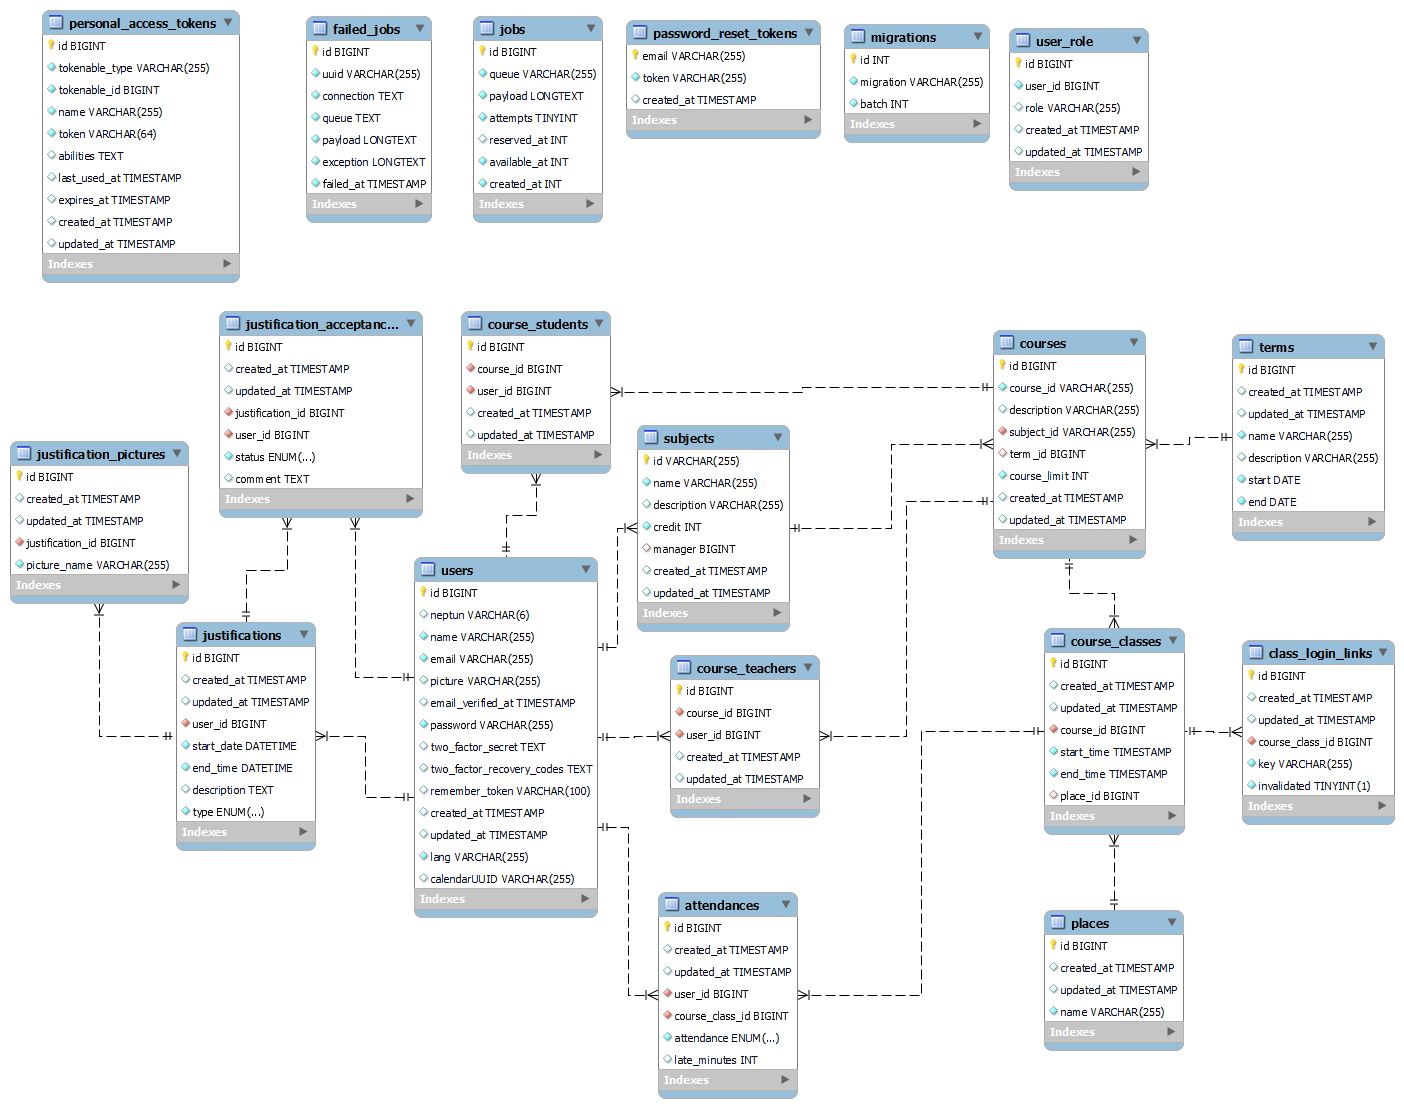
\includegraphics[width=15cm]{../pictures/db.png}
	\caption{Az alkalmazás által használt adatbázis.}
	\label{database}
\end{figure}

\begin{itemize}
	\item \emph{users, user\_roles}: ez a tábla tárolja a felhasználók adatait, illetve a felhasználókhoz tartozó jogosultsági köröket. Minden felhasználóról tárolunk egy azonosítót, egy Neptun\cite{Neptun} kódot\footnote{A neptun kód egy 6 karakter hosszú, egyedi azonosító.}, nevet, email címet, egy titkosított jelszót, egy profilképet, a felhasználó által használt nyelvet, illetve egy UUID-t\footnote{}, azaz egy egyedi azonosítót, amit az órarend exportálásához lehet használni, erről később. Az azonosító oszlopra azért van szükség, mivel az alkalmazás fel van készítve arra, hogy Neptun kód nélkül rendelkező felhasználókat is tudjon kezelni.
	\item \emph{terms, places}: a félévek és termek (helyek) tárolására szolgáló táblák.
	\item \emph{subjects, courses, course\_classe, class\_login\_links}: ezen táblák tárolják a tantárgyakat (amik többek között rendelkeznek egy azonosítóval, névvel, leírással, kreditértékkel, és egy tantárgyfelelőssel), a tantárgyakhoz tartozó kurzusokat (amihez tárolok egy azonosítót, ami minden esetben egyedi, egy kurzus azonosítót, ami minden félév és tantárgy esetében kell egyedinek lennie, tartozik hozzá egy félév, illetve egy létszám limit), illetve kurzusokhoz pedig órák (amiknek van egy kezdete, vége, illetve egy terem, ahol tartják). Az utolsó tábla pedig az órákhoz tartozó bejelentkező linkeket tartalmazza, ennek jelentőségéről kicsit később.
	\item  \emph{attendances}: itt tárolom az egyes kurzusok résztvevőinek az órai jelenléteit, melyek lehetnek: nincs kitöltve, jelen, késés (mely esetben percben lehet tárolni a mértékét), hiányzás, igazolt hiányzás.
	\item \emph{justification, justification\_acceptances, justification\_pictures}: ezek a táblák tárolják az igazolásokat, az igazoláshoz tartozó feltöltött képeket, illetve az igazolásban érintett tanárok válaszát, hogy elfogadják-e ó, vagy sem.
	\item Az egyéb, nem említett táblák inkább kapcsolótábla funkciót töltenek be, vagy a keretrendszernek vannak rá szükségei. Például a \emph{jobs} tábla a háttérben végrehajtandó feladatokat (job) tartalmazza.
\end{itemize}

Itt érdemes még megemlíteni, hogy a fejlesztés során a MySQL nevezetű, relációs adatbázist használtam, viszont a Laravel keretrendszerből adódóan sok más típusú adatbázis szoftverrel használható az alkalmazás, mivel a táblák felépítése a keretrendszer nyújtotta módon van elkészítve.

\section{Általános információk}

\subsection{Felhasználók}
\label{users}

Az alkalmazás 4 különböző jogkört különböztet meg a felhasználók esetén, melyekből egyszerre többet is birtokolhat a felhasználó:

\begin{itemize}
	\item Szuper adminisztrátor: képes a felhasználók adatainak -- és jogköreinek -- szerkesztésére, illetve az alkalmazás alapbeállításainak módosítására.
	\item Adminisztrátor: a félévek, termek, tantárgyak, kurzusok, órák, készítésére, módosítására, törlésére jogosult.
	\item Tanár: megtekintheti a tanított óráit, kurzusait, hallgatóit. Adminisztrálni tudja az órákon való részvételt, illetve megtekintheti és bírálhatja a hozzá érkezett igazolásokat.
	\item Hallgató: a hozzárendelt óráit, tantárgyait látja, megtekintheti minden kurzus esetén az egyes órák státuszát, illetve igazolásokat hozhat létre
\end{itemize}

Az alkalmazás természetesen rendelkezik bejelentkezés, regisztráció funkciókkal. A felhasználók Neptun\cite{Neptun} kódjuk vagy email címük, illetve a jelszavuk megadásával tudnak bejelentkezni. Regisztrálni csak abban az esetben tudnak, ha az oldal beállításaiban ezt engedélyezték, egyéb esetben a szuper adminisztrátorok tudnak felhasználókat létrehozni vagy importálni. Belépés után  a profil szerkeszthető, a jelszó cserélhető.

\subsection{Általános funkciók}

Bejelentkezés után a főoldalon a felhasználók pár, számukra fontos vagy érdekes információt láthatnak. Tanulók esetében a mai napi óráikat, illetve adminisztrálásra váró igazolásaikat. Tanárok esetén szintén a mai óráikat, illetve a kapott igazolásaikat láthatják. Az adminisztrátorok pár statisztikát láthatnak az oldal kapcsán.

\begin{figure}[ht!]
	\centering
	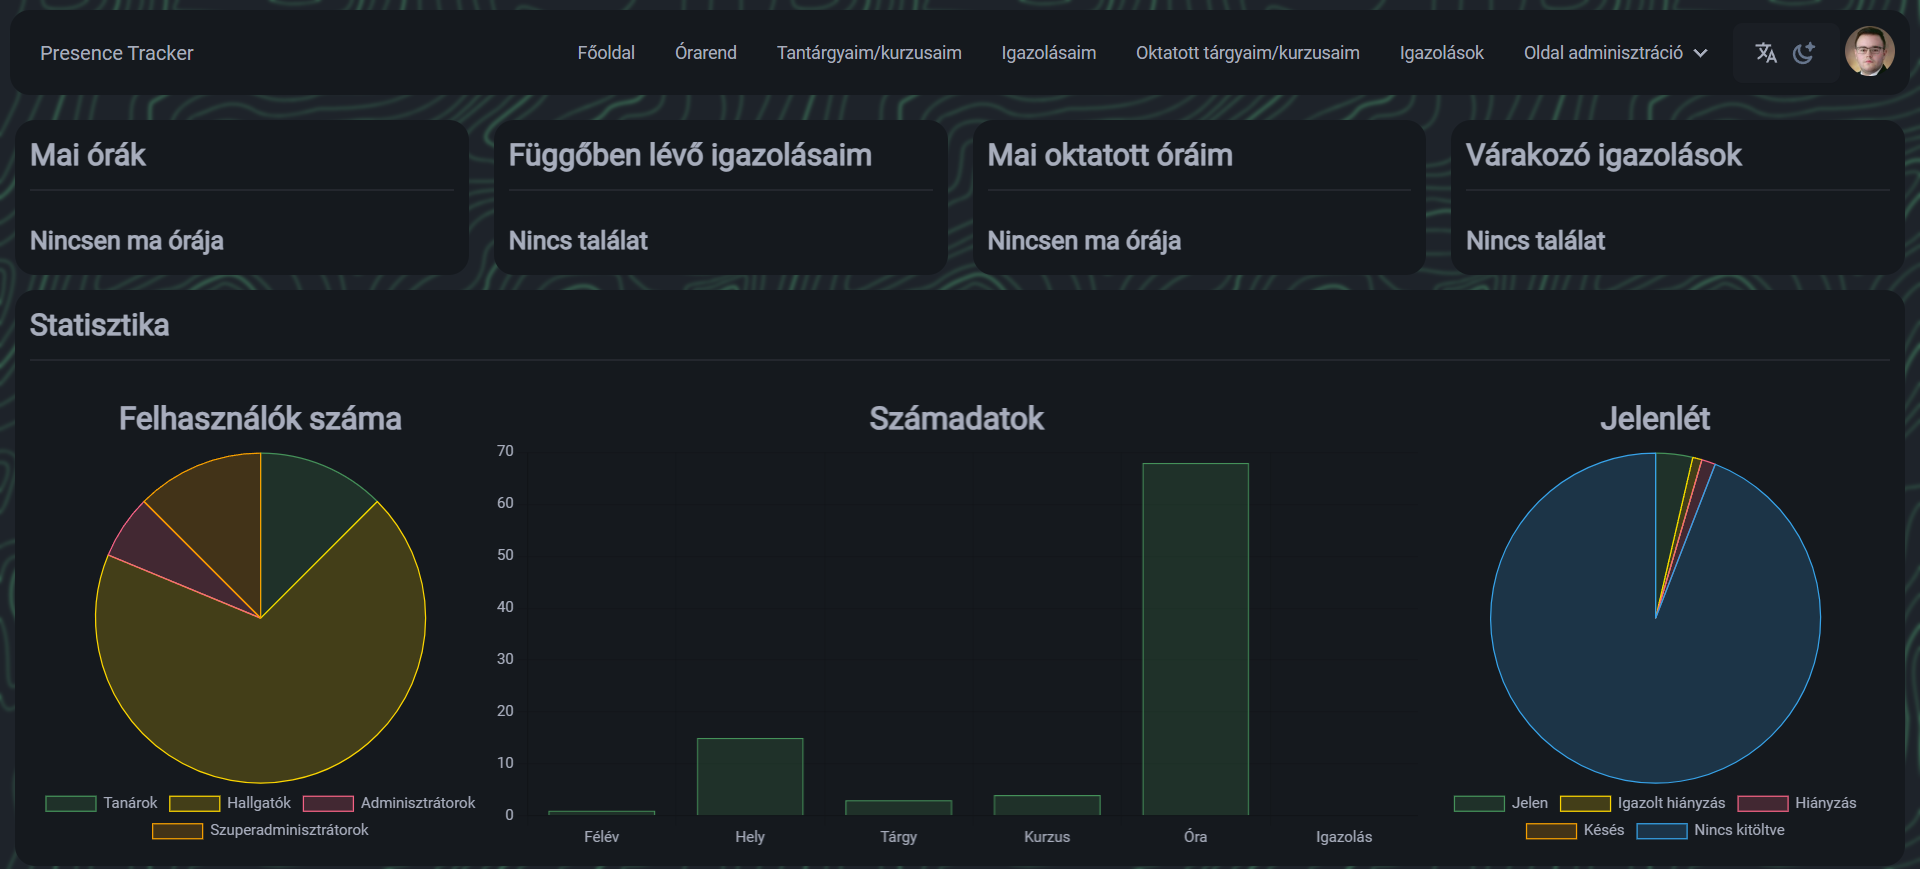
\includegraphics[width=10cm]{../pictures/screenshots/landing.png}
	\caption{A főoldal kinézete abban az esetben, ha a felhasználó minden szerepkörrel rendelkezik. A két bal oldali oszlop a hallgatói nézethez tartozik, a két jobb oldali pedig az oktatóihoz, míg a statisztika adminisztrátorok esetén jelenik meg.}
	\label{landing}
\end{figure}

A profil kép melletti gombra kattintva a felhasználó meg tudja változtatni az oldal nyelvét, Angol és Magyar nyelv közül választva, illetve az oldalt kinézetét: világos és sötét mód között váltogatva. A nyelv beállítása eltárolódik a felhasználóhoz, így újabb bejelentkezés esetén automatikusan beállításra kerül.

Tanuló vagy tanár esetén megjelenik az \emph{Órarend} menüpont is, ahol egy helyen láthatják a heti óráikat a felhasználók. Az egyes órák különböző színekkel jelennek meg, ezzel jelezve, hogy az adott órát a felhasználó tanítja-e, vagy hallgató esetén az órán jelen volt, hiányzott, késett, igazoltan hiányzott, vagy még nincs kitöltve a jelenlét. Lehetőség van az órarend exportálásra is, mely során egy \emph{.ics} kiterjesztésű fájl áll elő. Ez egy széles körben használt általános naptár formátum, amit a felhasználók be tudnak importálni a gyakorian használt naptár programokba\cite{ICS}. Ezáltal kedvenc naptár alkalmazásukban is nyomon tudják követni óráikat.

Lehetőség van a weboldalt alkalmazásként telepíteni, ahogy az \aref{install} ábrán is látható, így gyorsan hozzáférhetnek az alkalmazás funkcióihoz, egy ,,rendes'' alkalmazás érzését keltve ezzel. Ezt a PWA\footnote{Jelentése: Progressive Web App: egy olyan alkalmazás, ami webes technológiákat használ, de platform specifikus alkalmazásként viselkedik.\cite{PWA}} teszi lehetővé, melynek működésére későbbiekben térek ki.

\begin{figure}[ht!]
	\centering
	
\includegraphics[width=8cm]{../pictures/screenshots/install.png}
	\caption{Az oldal telepítésére szolgáló felugró ablak.}
	\label{install}
\end{figure}

\section{Adminisztrátori nézet, funkciók}

\subsection{Felhasználók kezelése}

Szuper adminisztrátor esetén a felhasználó képes kezelni az alkalmazásban tárolt felhasználókat, kivéve saját magát (személyes adatait továbbra is meg tudja változtatni). A listában képes szűrni a felhasználók között, megváltoztatni profil adataikat, jelszavukat alaphelyzetbe állítani, szerkeszteni jogosultsági szintjeiket, illetve akár törölni is őket, ha szükséges. Tud új felhasználókat létrehozni, illetve képes fájlból is importálni adatokat.

\subsection{Alkalmazás konfiguráció}

Szintén a szuper adminisztrátor körébe tartozik az oldal beállításainak kezelése. Az alábbi beállításokat tudja kezelni:
\begin{itemize}
	\item Oldal neve: az oldalon megjelenő név megváltoztatása.
	\item Regisztráció engedélyezése: ezzel lehet engedélyezni, hogy a felhasználók maguktól is tudjanak-e felhasználói fiókot készíteni az oldalon.
	\item Saját Neptun\cite{Neptun} kód megváltoztatása: beállítható, hogy a felhasználó meg tudja magának változtatni ezt az értéket, vagy sem.
	\item Kötelező Neptun kód: az oldal használható ezen kód megadása nélkül is, ez itt szabályozható.
	\item Alkalmazás képe: itt tölthető fel új kép, ami a fő oldalon jelenik meg látogatók esetén.
\end{itemize}

\subsection{Félévek, termek, tantárgyak, kurzusok, órák kezelése}

Minden adminisztrátor képes ezen adatok kezelésére.

Félévek esetén egy nevet, illetve egy kezdő és vég dátumot szükséges megadni. Ellenőrizve van, hogy a félévek nem ütközhetnek egymással. A listában egy pipa jelzi a jelenlegi félévet, ha van ilyen.

A termeknél elegendő egy nevet megadni, ezeket lehet az egyes órákhoz hozzárendelni.

Tantárgyak esetén egy tárgy kódot, egy nevet, egy opcionális leírást, egy kredit értékéket, illetve egy tantárgyfelelőst tárol, akinek rálátása van a tárgy összes kurzusára. Ezen belül minden kurzus egy tárgyhoz kapcsolódik. Ezek szintén rendelkeznek egy kóddal, ami minden tárgy és félév esetén egyedi, szintén egy opcionális leírással, illetve nulla, egy, vagy több tanárral. Minden kurzus egy félévhez van rendelve. A kurzusokhoz hozzárendelhetők a hallgatók, és csak hallgatók.

A kurzusokhoz órák hozhatóak létre, amik a féléven belül lehetnek. Minden óra külön kezdés és vég időponttal rendelkezik, illetve egy teremmel, ahol tartják. Az óra létrehozásakor lehetőség van arra is, hogy a félév végig heti ismétléssel hozza létre az órákat -- természetesen később egyenként lehet őket szerkeszteni, törölni --, ezáltal megkönnyítve az adminisztrációt.

\begin{figure}[ht!]
	\centering
	
\includegraphics[width=15cm]{../pictures/screenshots/newclass.png}
	\caption{Új óra hozzáadása.}
	\label{newclass}
\end{figure}


\section{Tanári nézet, funkciók}

\subsection{Oktatott tárgyak}
\label{taugthClass}

A tanárok megtekinthetik az általuk oktatott -- vagy tantárgyfelelősként hozzáadott -- tárgyakat, és az azokhoz kapcsolódó adatokat. Igény szerint szűrhetnek kód, név, vagy félévre is. Minden kurzus esetén megtekinthetik az alap adatokat, a kurzushoz tartozó órákat, hallgatókat. Itt van lehetősége a tanárnak hozzáadni hallgatókat a kurzushoz, illetve egy listában megtekinteni diákokra lebontva, hogy mennyit hiányoztak, mennyit késtek, ebből mennyi az igazolatlan.

A kurzus órái listában érhetik el az egyes órákat, ahol adminisztrálhatják a jelenlétet. Egy órát megnyitva láthatják az ahhoz kapcsolódó adatok, illetve bal oldalon egy listát a kurzus tanulóiról, ahol beállíthatják a hallgató státuszát. Amennyiben az adott hallgató a tanár által elfogadott igazolással rendelkezik, akkor ebben az esetben csak ,,jelen'' státusz -- ha esetleg mégis megjelent az órán --, vagy pedig ,,igazol hiányzás'' státusz állítható be, illetve egy figyelmeztető üzenet is megjelenik. Ezek mellett megjelenik az adott kurzuson való összes hiányzás és igazolt hiányzások száma is. Hiányzás rögzítése esetén email üzenet formájában is értesítést kap a hallgató.

A jobb oldalt kettő doboz foglal helyet. Az első egy Qr\footnote{A Qr kód egy információt tartalmazó kép,  amit kamerával lehet leolvasni.\cite{QR}} kódot tartalmaz. Ennek segítségével, ha az oktató látható teszi, a diákok a kódot a telefonjukon beolvasva, majd bejelentkezve is ,,beírhatják magukat'' az órára, ezzel felgyorsítva a folyamatot, és a tanárnak sem kell végig mennie a listán. A kód csak az óra végéig működik, illetve ha az oktató úgy sejti, hogy a hallgatók visszaélnek ezzel, akkor hamarabb is letilthatja, illetve generálhat egy másikat. Amikor a hallgató íj módon bejelentkezik az órára, a tanári felületen automatikusan frissítésre kerül a státusz. A hallgató csak abban az esetben tudja ezt a funkciót használni, hogy ha fel van iratkozva a kurzusra, és még nem állították be az adott órára a státuszát, ezzel elkerülve, hogy magától átírja esetleges hiányzását, késését.

A másik ilyen doboz egy kis statisztikát mutat kör diagram formájában, megszámolva a hallgatók státuszát az órán.

\begin{figure}[ht!]
	\centering
	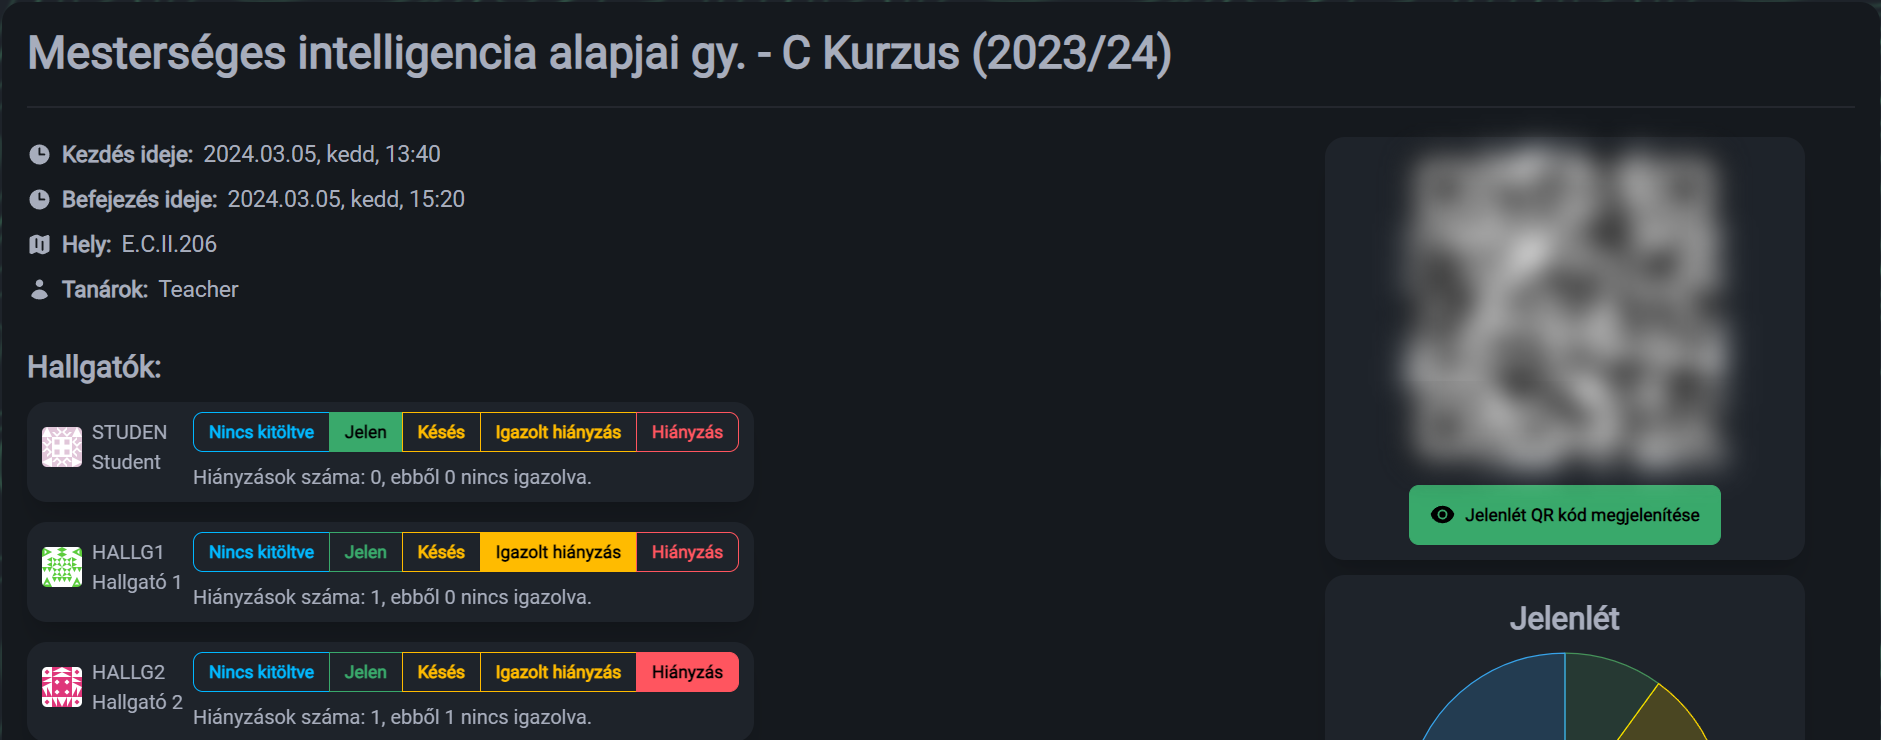
\includegraphics[width=10cm]{../pictures/screenshots/class_1.png}
	\caption{Egy óra nézete.}
	\label{class}
\end{figure}

\begin{figure}[ht!]
	\centering
	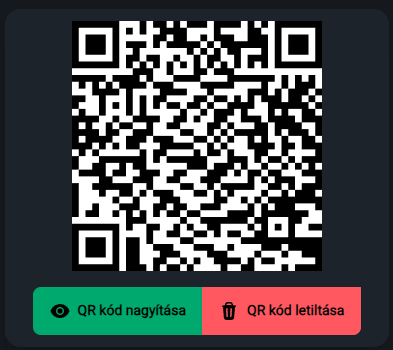
\includegraphics[width=6cm]{../pictures/screenshots/class_2.png}
	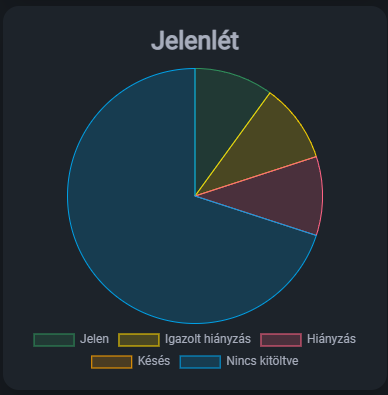
\includegraphics[width=6cm]{../pictures/screenshots/class_3.png}
	\caption{Egy óra kártyái.}
	\label{class2}
\end{figure}

\subsection{Igazolások}

Amikor egy hallgató igazolást ad le, akkor azt minden érintett tanár megkapja, és reagálhat rá; vagy elfogadja, vagy indoklással elutasítja. A lista alapból szűrésre kerül, hogy csak a még nem meg válaszolt igazolásokat mutassa az oktatónak. Amikor a tanár megnyit egy ilyen igazolást, láthatja, hogy ki küldte be az igazolást, a típusát (orvosi vagy egyéb), az kezdeti és vég időpontot, illetve az esetlegesen feltöltött képeket is megtekintheti. Ezek mellett listába szedve, és tantárgy, majd kurzus alapján kategorizálva látja az általa oktatott és az igazolásban érintett órákat, azok idejét, illetve a hallgató jelenlegi státuszát az órán. Az igazolás elfogadása esetén azon órák, ahol nem ,,jelen''-re van állítva az állapot, automatikusan ,,igazolt hiányzás'' állapotra kerülnek beállításra. Elfogadás és elutasítás esetén is üzenet kap a hallgató, illetve a főoldalon megtekintheti a még függőben lévő (tehát nem minden érintett tanár által megválaszolt) igazolásait is.

\begin{figure}[ht!]
	\centering
	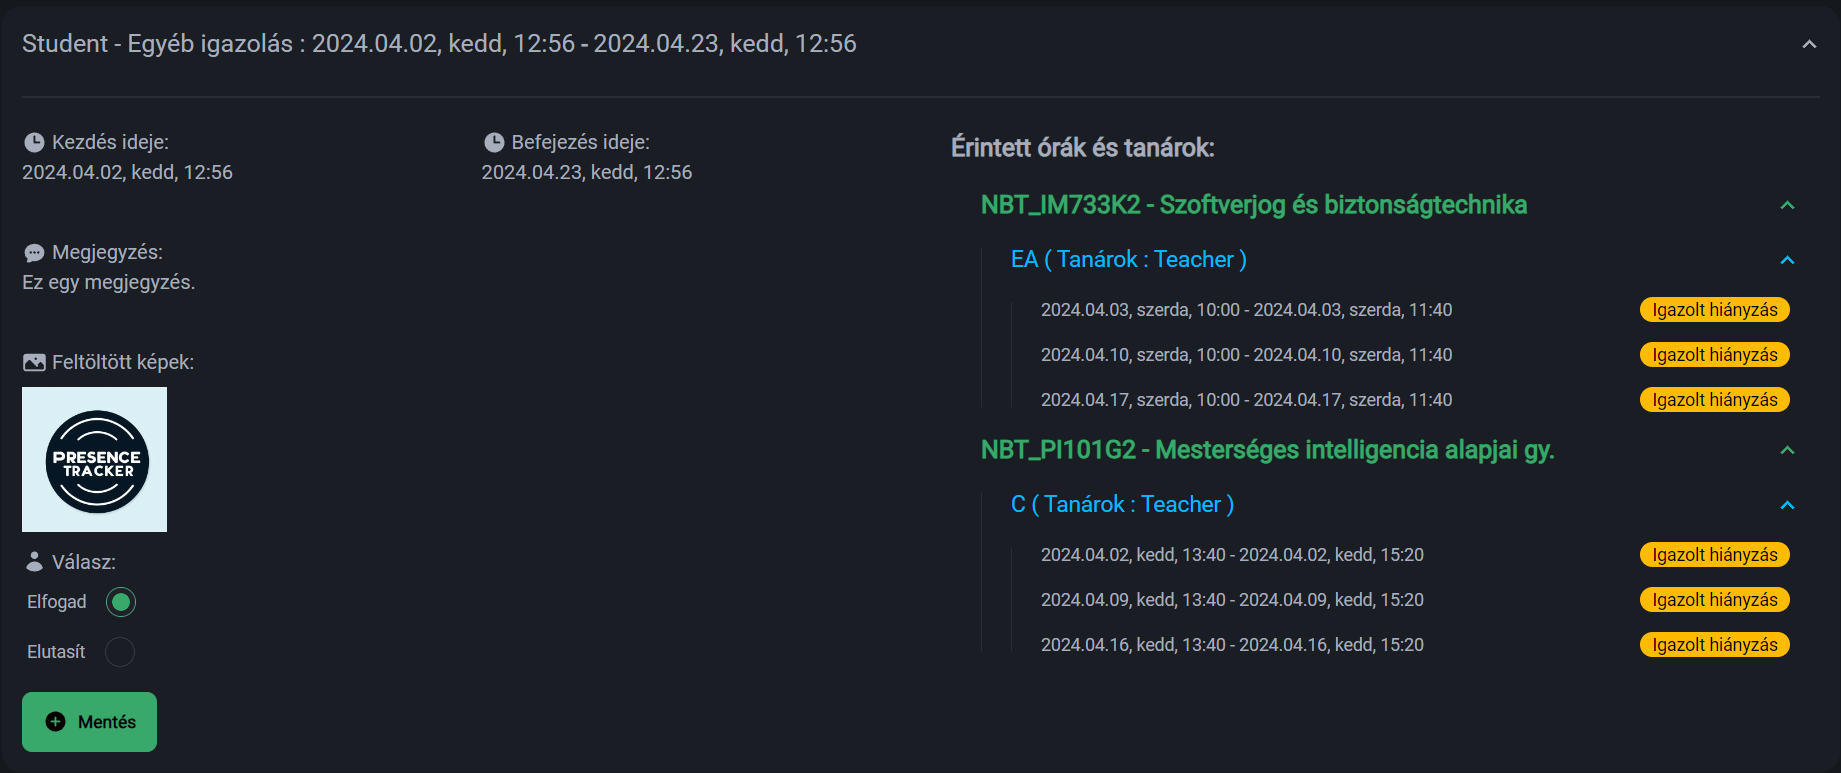
\includegraphics[width=15cm]{../pictures/screenshots/just_teacher.png}
	\caption{Egy elfogadott igazolás, ahogy a tanár látja.}
	\label{justTeacher}
\end{figure}

\section{Hallgatói nézet, funkciók}

\subsection{Tantárgyak, kurzusok}

A hallgatók természetesen láthatják a tantárgyaikat, amiket csakugyan szűrhetnek név, kód, félév szerint. Itt egy helyen megtekinthetik kurzusokra lebontva, hogy melyik órán milyen státusz van rögzítve, illetve egy diagramon ezeknek az eloszlását. Megtekinthetik még a kurzuson lévő hallgatótársaikat is.

\begin{figure}[ht!]
	\centering
	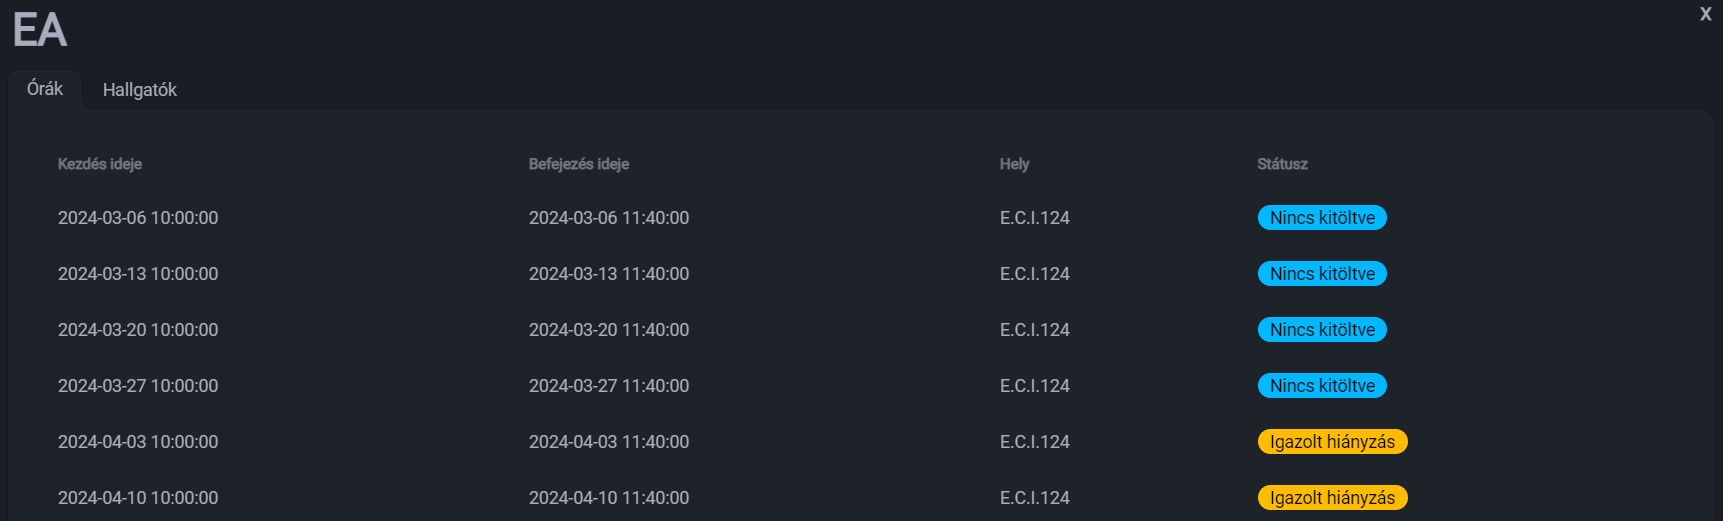
\includegraphics[width=12cm]{../pictures/screenshots/student_course.png}
	\caption{A hallgató által látott egy kurzus részlete.}
	\label{studentCourse}
\end{figure}

\subsection{Hallgató által létrehozott igazolások}

A hallgató a hiányzásainak igazolására igazolásokat adhat le a rendszerben. A létrehozáskor meg kell adnia a típusát (orvosi vagy egyéb), a kezdeti és vég dátumát, illetve szükség szerint megjegyzést fűzhet, illetve képeket tölthet fel, például az orvosi igazolást lefényképezheti. A dátumok megadása után a hallgató is látja az érintett óráit listába szedve.

Helyes adatok megadása és mentés után a listában is megjelenik az igazolás, amit lenyitva látja a megadott részelteket, illetve az egyes tanárok visszajelzését is, hogy elfogadták-e vagy sem. Amennyiben úgy látja, hogy elrontott valamit, akkor itt törölheti az igazolást, és hozhatja újra létre.

\begin{figure}[ht!]
	\centering
	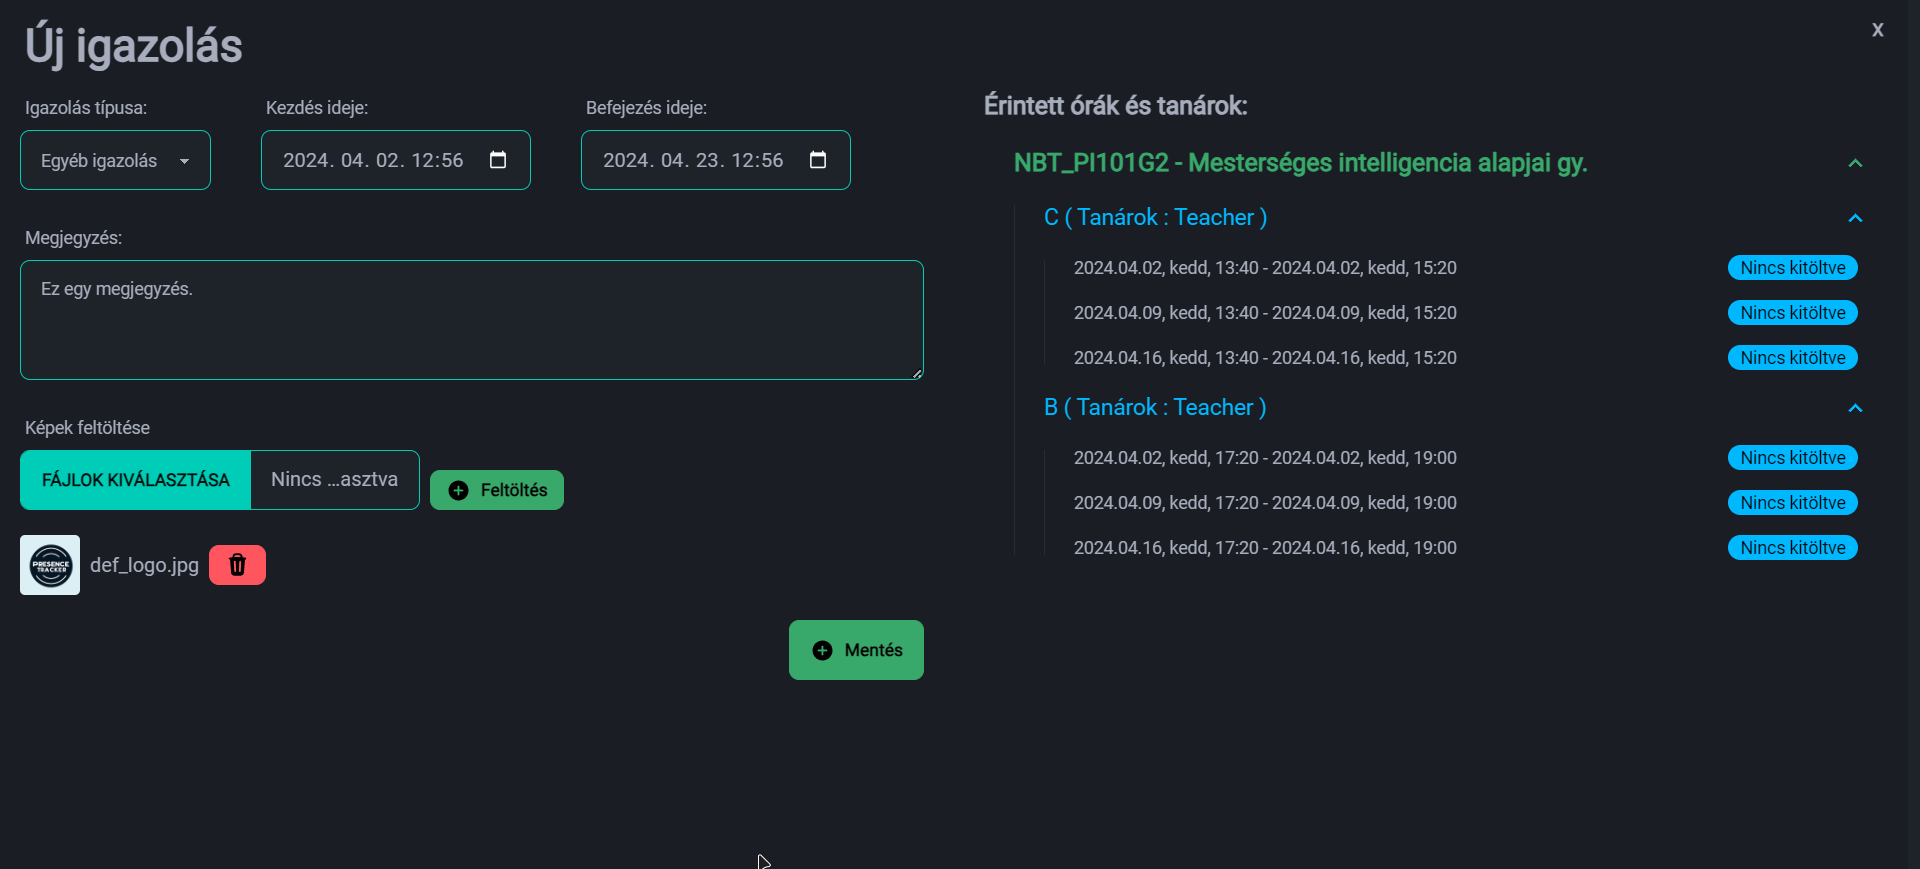
\includegraphics[width=12cm]{../pictures/screenshots/newJust.png}
	\caption{Új igazolás létrehozása képernyő.}
	\label{studentJustification}
\end{figure}

\chapter{Felhasznált technológiák, csomagok}
\label{packages}
\section{Laravel}

Ahogy a bevezetőben említettem, a megvalósításhoz a Laravel nevezetű keretrendszert használtam. A keretrendszer sok funkciót alapból elkészít, amit hosszadalmas lenne újra és újra megírni, ezáltal a programozó a lényegre fókuszálhat: az elkészítendő programra.\cite{meetlaravel}

\subsection{Keretrendszer alapjai}

\subsubsection{MVC architektúra}

A keretrendszer az MVC architektúrát követi, ami segíti a kód karbantartását, áttekinthetőségét.\cite{mvc} Ez azt jelenti, hogy logikailag a kód három része bomlik:
\begin{itemize}
	\item Modellek (Model): ezek tartalmazzák az adatbázis táblák modelljeit, ezeken keresztül tudjuk elérni az adatbázisunkat, illetve az adatbázisban tárolt adatokat is modellek formájában kapjuk meg, így ezeknek követni kell a táblák felépítését. Ezek mellett kapcsolatokat is meg tudunk adni a modellek között.
	\item Nézet (View): itt magára a nézetekre kell gondolni, amit látni fog a felhasználó. Ezek jelen esetben a Blade\cite{blade} fájlok, amire \aref{bladeSection}. alfejezetben térek ki.
	\item Kontroller (Controller): az üzleti logikát tartalmazza. Itt kapnak helyet a függvények például, amik egy kérés fogadásakor futnak le.
\end{itemize}

\subsubsection{Útvonalak}

A keretrendszerben az útvonalakat a \emph{routes} mappában található fájlokban találjuk. Mivel a keretrendszer képes nem csak webes kéréseket kiszolgálni, így több fájlra vannak szedve, viszont én csak a webes útvonalakhoz tartozó fájlt használtam.

Útvonalakat a \emph{Route} osztály metódusaival tudunk létrehozni. Ezek után meg kell adnunk a útvonal típusát (tehát hogy \emph{Get, Post, Put vagy Delete} típusú útvonalat szeretnénk létrehozni), magát az elérési útvonalat, illetve a meghívandó programkódot, ami ki fogja szolgálni a kérést. Opcionálisan megadhatunk egy nevet is, amivel referálni tudunk rá a kódunk többi részéből, illetve adhatunk meg egy vagy több köztes program kódot (angolul: middleware), mellyel kontrollálhatjuk az útvonal elérést és egyéb más dolgokat tehetünk meg a kérés kiszolgálása előtt.\cite{routing} Erre láthatunk egy példát \aref{routesandMiddleware} kódban.

Amennyiben az olvasó megnézi az elkészült programban található útvonalakat, azt láthatja, hogy csak \emph{Get} típusú útvonalak találhatóak benne. Ennek fő oka a Livewire\cite{livewire} használata, ahol útvonalak létrehozása helyett metódushívásokkal történik sok interakció, erről \aref{livewireSection}. alfejezetben lesz szó.

\subsubsection{Middleware}

A middleware arra alkalmas, hogy a kérés feldolgozása előtt végezzünk el teendőket, akár szűrjük őket.\cite{middleware} A program során én három fő dologra használtam ezt fel: bejelentkezés vizsgálata, hozzáférési jogosultság vizsgálata, illetve a kérés elején az alkalmazás nyelvének beállítása. Az utolsóra azért volt szükség, mivel Laravel esetén a nyelv beállítása mindig csak az adott kérésre vonatkozik. Így minden esetben meg kellett vizsgálni, hogy a felhasználó átállította-e a nyelvet, és ha igen, akkor alkalmazzuk a kiválasztott nyelvet a kérésre. A middleware futása során dönthetünk úgy is, hogy a kérést megszakítjuk, például ha a felhasználó nem rendelkezik kellő jogosultsággal. Hozzá is tudjuk rendelni ezeket az egyes útvonalakhoz, ahogy az \aref{routesandMiddleware}. kódrészleten látható, vagy akár beállíthatjuk, hogy globálisan, minden kérés esetén lefusson az adott kód. \Aref{middleware}. kódrészletben egy middleware-ből látható egy részlet, ami adminisztrátorok esetén engedélyezi a kérést.

\lstinputlisting[caption={Egy \emph{Get} típusú útvonal, ami az órarendet nyitja meg. Az útvonal meghívásakor a \emph{Controller} nevű osztály \emph{getTimetable} metódusa fut le. Az útvonalat csak bejelentkezett felhasználók ('auth') és diákok vagy tanárok ('studentorteacher') érhetik el.}, label=routesandMiddleware, style=php]{../codes/route.php}

\subsubsection{Konfiguráció}

A \emph{config} mappában találhatók a konfigurációs fájlok. Ha jobban megnézzük, ezek igazából PHP fájlok, amik egy tömb-ként adják vissza a konfigurációs értékeket. Ezeket módosíthatjuk, illetve mi is hozhatunk újakat létre. Én is így tettem: az olyan beállításokat, mint például, hogy engedélyezve van-e a regisztráció, vagy hogy a felhasználók módosíthatják-e a kódjukat, innen kérdezem le. Sok esetben az értékeket a környezeti konfigurációs fájlból olvassa be a program, ezáltal a gyakran változó értékek egy helyen módosíthatók anélkül, hogy keresni kéne őket, hogy hol vannak.

\subsubsection{Nyelvesítés}

Az alkalmazás két nyelvet támogat jelenleg: Angolt és Magyart, ezekhez készítettem el a fordítást. A nyelvesítést tartalmazó fájlokat a \emph{lang} mappában találhatjuk, nyelvek szerint almappákra bontva. Az egyes kifejezések kulcs-érték párokként vannak eltárolva, ezen kulcs segítségével tudjuk elérni őket a \emph{\_\_('kulcs')} segédfüggvény segítségével, ami globálisan elérhető a Kontroller és a Nézet fájlokban is. A keretrendszer automatikusan a beállított nyelv alapján visszaadja a megfelelő fordítást. Ha esetleg hiányozna az egyik fordítás, akkor a konfigurációban alapértelmezettként megadott nyelvből próbálja kikeresni az értéket. Ha ott sem találja meg, akkor a paraméterként megadott kulcsot adja vissza.

\subsection{Adatbázis és modellek}

Az adatbázis felépítése a keretrendszer adta módon van megoldva. Ez azt jelenti, hogy minden, a Laravel által támogatott adatbázis disztribúcióval működni fog a felépített adatbázis séma. A táblák úgynevezett migrációk segítségével vannak leírva. Ez egyrészt segíti az adatbázis megosztását a fejlesztők között, hiszen nem kell külön adatbázis fájlokat küldözgetni egymás között, másrészt egyfajta verziókezelést tesz lehetővé: hogyha valamit módosítunk az adatbázison, akkor új migrációt hozunk létre. Amikor egy másik fél letölti a változtatásokat, és elindítja a migrációt, a keretrendszer felismeri melyik változtatásokat kell alkalmaznia, és melyek azok, amik már alkalmazva lettek.\cite{migrations}

\subsubsection{Migrációk}

A migrációk a \emph{database} mappán belül a \emph{migrations} mappában találhatók. Egy fájl általában egy tábla leírását vagy módosítását tartalmazza a jobb átláthatóság érdekében. Minden migráció két eljárást tartalmaz: az \emph{up()} eljárás az adatbázis migráció futtatásakor fut le, míg a \emph{down()} az adatbázis törlése vagy teljes újraépítése esetén, tehát az előbbi eljárás ellentettjét végzi el.\cite{migrations}

A táblákat a \emph{Schema} osztály \emph{create} metódusával tudjuk létrehozni. Ez két paramétert vár: a tábla nevét, illetve a tábla felépítését leíró függvényt. Ezen függvény belül írhatjuk le a tábla mezőit.

\Aref{migrationCode}. kódrészletben egy ilyen migrációt láthatunk, ahol egy kurzusok tárolására szolgáló táblát hozom létre. Itt több, különböző mező létrehozása megfigyelhető:
\begin{itemize}
	\item Az egyik első lépés szokott lenni a tábla elsődleges kulcsának meghatározása. Éppen ezért a Laravel biztosít erre egy gyorsabb módszert: a második sorban látható \emph{\$table->id()} segítségével létrehozható egy id nevű, szám típusú, automatikusan növekvő mező.
	\item Természetesen sima mezőket is létrehozhatunk, ehhez a típusát, a nevét, és egyéb opciókat adhatunk meg, mint például az alapértelmezett értékét, vagy hogy a mező null-ra állítható-e. Ilyet például a negyedik vagy a nyolcadik sor.
	\item Tudunk idegen kulcsokat is definiálni, ahogy azt a hatodik és hetedik sorban láthatjuk. Ehhez a \emph{foreign()} függvényt kell használni, megadni a mező nevét, illetve hogy melyik tábla melyik mezőjét referáljuk ezzel az idegenkulccsal. Megadható az is, hogy törlés vagy módosítás esetén mi történjen. A példán egyik esetben törlése kerül a rekord, más esetben null-ra állítódik a mező.
	\item Laravel esetében szokás két dátumot is adni a táblákhoz: egyet, hogy mikor jött létre az egyed, és egyet, hogy mikor módosították utoljára. Ezt könnyen meg lehet tenni a kilencedik sorban látható módon.
\end{itemize}

\lstinputlisting[caption={A kurzusokat tároló tábla migrációja.}, label=migrationCode, style=php]{../codes/migration.php}

Lehetőségünk van már létező táblákat módosító migrációt is írni. Ilyenkor a \emph{create} helyett a \emph{table} függvényt kell használni. A \emph{down()} függvény általában a tábla törlésére szolgáló kódsort tartalmazza.

\subsubsection{Modellek}

Az adatbázis modellek a \emph{app} könyvtáron belül a \emph{Models} mappában találhatók. Minden modellt egy osztállyal lehet leírni. Amennyiben követjük a Laravel elnevezési konvencióját\cite{tableNames}, akkor nem szükséges megadnunk a modellhez kapcsolódó tábla nevét, egyébként igen.

A modellen belül megadhatunk több információt, mint a tábla neve, ha szükséges, illetve beállíthatjuk, hogy az elsődleges kulcs az automatikusan növekedjen-e vagy sem. Megadhatjuk azt is, hogy mely mezőket lehet kitölteni a \emph{\$fillable} mező segítségével. A \emph{\$hidden} mezővel megadhatjuk, hogy mely attribútumokat nem szeretnénk szerializálni (ilyen lehet például a jelszó), és azt is megadhatjuk, hogy ha egyes adatbázis mezőket szeretnénk átkonvertálni más típusúra (ilyen például ha a tárolt dátumot a keretrendszer által biztosított dátum objektummá szeretnénk alakítani). Az adatbázis mezőit ezeken felül nem kell megadnunk, azokat úgynevezett ,,magic method''-on\cite{magicMethod} keresztül tudjuk elérni.

A másik nagyobb ,,kategória'', amit meg szoktak írni a modellek esetén, azok a kapcsolatok. A keretrendszer lehetőséget nyújt a szokásos kapcsolatok (egy az egyhez, egy a többhöz stb.) kialakítására függvények segítségével. \Aref{onetomany}. kódrészletben egy a többhöz kapcsolatot lehet látni. \Aref{manytomany}. kódrészletben pedig egy több a többhöz kapcsolatot, ami kettő, egy a többhöz kapcsolattal van feloldva, ahol a kapcsoló tábla a \emph{course\_students}. Érdemes megfigyelni, hogy nincsenek megadva a kapcsolatoknál az azokat megvalósító idegenkulcsok nevei. Ahogy az fentebb említettem, ha követjük az elnevezés konvenciót, akkor azokat itt sem kell megadni. Ez alól a több a többhöz kapcsolat esetén a kapcsolótábla neve jelent kivételt.

\lstinputlisting[caption={Egy a többhöz kapcsolat: egy tantárgynak több kurzusa van.}, label=onetomany, style=php]{../codes/onetomany.php}
\lstinputlisting[caption={Több a többhöz kapcsolat: egy kurzusnak több hallgatója van, egy hallgató több kurzusra van felíratkozva.}, label=manytomany, style=php]{../codes/manytomany.php}

\subsection{Eloquent ORM}

Az ORM, avagy az Object Relational Mapping rendszerek abban nyújtanak segítséget, hogy összekössék az adatbázist a modelljeinkkel, ezáltal a modelleket használhatjuk az adatbázissal való kommunikáció során SQL parancsok írása helyett.\cite{orm} A Laravel egy nagyszer ORM rendszerrel készül, amit Eloquent-nek\cite{eloquentORM} hívnak. Segítségével bonyolult lekérdezéseket, frissítéseket, létrehozásokat tudunk elvégezni a modelleken keresztül. Bár a bonyolultabb lekérdezések megírása elsőre nehézséget jelentett, könnyen megtanulható és megszokható volt ez az ORM, és gyorsan meg is szerettem.

\Aref{eloquent} kódrészletben egy ilyen lekérdezést láthatunk: lekérdezem a tantárgyakat, illetve szűröm őket, ha adott meg szűrési feltételeket a felhasználó. Emellett látható az is, hogy a lapozás is keretrendszer szinten támogatott a \emph{paginate} függvény segítségével. Ehhez meg kell adni, hogy hány elemet szeretnénk megjeleníteni egy oldalon, és opcionálisan egy nevet is adhatunk neki, ami akkor hasznos, ha több ilyen lapozó szakaszt is tartalmaz az oldal. 

\lstinputlisting[caption={Tantárgyak lekérdezése, szűrése ha adtak meg értéket.}, label=eloquent, style=php]{../codes/eloquent.php}

\subsection{Blade sablon fájlok}
\label{bladeSection}

A nézetek és komponensek létrehozására is megoldást nyújt a keretrendszer a Blade\cite{blade} fájlok formájában. Ezek szokványos HTML kódot tartalmaznak, illetve a Blade által nyújtott direktívákat, de akár egyszerű PHP kódot is tartalmazhat, mivel végső soron ezekből PHP fájlokat készít a keretrendszer.

A Blade különböző direktívák használatát teszi lehetővé, ami megkönnyíti a nézetek létrehozását. Ezek általában egy \emph{@} jellel kezdődnek. Segítségükkel feltételeket rakhatunk a HTML kódunkba, ciklusokat a kollekciók kiíratására, de például gyors megoldást ad arra is, hogy az oldal egyes részeit csak bejelentkezett felhasználóknak jelenítsük meg a \emph{@auth} direktíva segítségével, csak hogy párat említsek. Ilyen direktívák láthatók \aref{directives}. kódrészletben példaképpen.

\lstinputlisting[caption={Bejelentkezett felhasználó esetén a jelenleg nem aktív félévek nevének kiíratása.}, label=directives, style=php]{../codes/directives.blade.php}

Hasznos segítséget nyújt a kinézet felépítésében is: az egyes nézetek kibővíthetnek másik nézeteket, ezáltal könnyedén létrehozható egy egységes nézet, mivel a főbb formázásokat és részleteket (például a navigációs sávot) elegendő egyszer megírni, a többi oldalunkat pedig ebből a fájlból kiterjeszteni.

Ezek mellett komponenseket is létrehozhatunk, amik újra és újra felhasználóható kódokat tartalmaznak. Én ezt első sorban az ikonoknál használtam ki, a többi esetben egy speciális, Livewire komponenseket használtam, erről többet \aref{livewireSection}. alfejezetben olvashatnak. Minden olyan ikon esetében, amit többször használtam, egy komponenst hoztam létre neki, ami tartalmazta a ikont leíró SVG kódot, így azt csak be kellett hivatkozni, ahogy az \aref{component}. kódrészletben látható. A komponens egy HTML tag-ként jelenik meg, illetve egy \emph{x-} előtaggal rendelkezik.

\lstinputlisting[caption={Komponens meghívása.}, label=component, style=php]{../codes/component.blade.php}

\subsection{Autentikáció}
\label{fortifyAuth}

A modellek és az adatbázis elkészítése után az egyik első dolgom volt az autentikáció kialakítása. Ez egy elég repetitív folyamat tud lenni, ezért ennek felgyorsítására a \emph{Laravel Fortify}\cite{fortify} nevű csomagot alkalmaztam.

Ezen csomag abban nyújt segítséget, hogy előre elkészíti az autentikációhoz szükséges útvonalakat, funkciókat, mint a bejelentkezés, regisztráció, jelszó visszaállítás. Magát a nézetek továbbra is nekünk kell létrehozni, illetve szükség esetén személyre szabhatjuk a különböző folyamatokat is. Gondolok itt arra, ha mondjuk nem email cím segítségével jelentkeznek be a felhasználók (például az én programomban beléphetnek email vagy Neptun kód segítségéve is), vagy ha több mezőt kell megadni regisztrációkor, mint amit a Fortify alapértelmezetten felajánl.

Amennyiben egy egyszerűbb alkalmazást készítünk, akkor lehetőségünk van használni több olyan csomagot, amik telepítéstől kezdve egy félkész alkalmazást adnak, amiben sok általános funkció (bejelentkezés, felhasználókezelés stb.) alapból el vannak készítve. Bár csábítóan hangzik, véleményem szerint ezeket nem érdemes használni, mivel egy nagyon általános, nem túl egyedi élményt nyújtanak, amit nehézkes lehet személyre szabni. Emiatt döntöttem inkább a Fortify használata mellett, és alakítottam ki a én a nézeteket.

\subsection{Jogosultság kezelés}

\subsubsection{Szerepkörök}

Ahogy azt \aref{users}. alfejezetben említettem, több szerepkört különböztetek meg a programban: szuper adminisztrátor, sima adminisztrátor, tanár és hallgató. Ezeknek a gyors létrehozására a Laravel Ladder\cite{ladder} csomagot alkalmaztam. Ennek segítségével gyorsan definiálhatók szerepkörök. A felhasználó modellt módosítja úgy a csomag, hogy gyorsan letudjuk ellenőrizni, hogy milyen szerepkör(ökk)el rendelkezik a felhasználó. Ezt elsősorban három helyen használtam: a middleware-ek esetén, hogy egy útvonal kinek elérhető, a nézetekben, hogy mely menüpontokat jelenítsem meg a felhasználónak, és a Policy-k esetén, erről bővebben lentebb.

\lstinputlisting[caption={Admin middleware részlet: az ez által védett útvonalak csak adminoknak érhetők el.}, label=middleware, style=php]{../codes/middleware.php}

\subsubsection{Jogosultság ellenőrzése}

Ahogy azt fentebb említettem, a middleware csak az egyik hely, ahol a szerepköröket használtam. A Policy-k\cite{policies} segítségével egy helyre lehet gyűjteni, hogy a felhasználó egy adott modell esetén milyen jogokkal rendelkezik: megtekintheti, újat hozhat lére, esetleg módosíthatja vagy törölheti. Minden modellhez készíthető ilyen szabály, egyszóval itt lehet definiálni a felhasználó jogait. Ez nálam a legtöbb esetben úgy nézett ki, hogy adminisztrátor (vagy szuper adminisztrátor) esetén mindenhez joga van, a modellek megtekintéséhez be kell jelentkezni, többi esetben a szituációtól függ a dolog, például tantárgyakat csak adminisztrátorok tudnak létrehozni, kezelni, de bármely bejelentkezett felhasználó megtekintheti.

\Aref{policyPart}. kódban egy részletet láthatunk a jogosultság vizsgálatra: a \emph{before} függvény minden függvény előtt lefut, itt vizsgálom meg, hogy adminisztrátorról van szó. Ha nem, akkor megy tovább a vizsgálat. Megtekinteni mindenki megtudja, létrehozni pedig csak adminisztrátor tud, viszont ezt már az előbb említett függvény levizsgálja, így itt elegendő egy hamis értéket vissza adni. \Aref{check}. részletben pedig magát a vizsgálatot láthatjuk egy konkrét esetben: a felhasználó rendelkezik egy \emph{can} és a fordítottja, egy \emph{cannot} függvénnyel, ezekkel lehet eldönti, hogy van-e jogosultsága a felhasználónak az adott művelethez, vagy sem. Ha nincs, akkor megjelenítek egy hibaüzenetet, és visszalépek a függvényből.
\pagebreak

\lstinputlisting[caption={Részlet a tárgyakhoz tartó szabályból.}, label=policyPart, style=php]{../codes/policies.php}

\lstinputlisting[caption={Jogosultság vizsgálata tárgy létrehozásakor.}, label=check, style=php]{../codes/authcheck.php}

Ezen szabályok nagy előnye, hogy ha bármely okból kifolyólag módosítani kell a kialakított szabályrendszeren, akkor ezt csak egy helyen kell megtenni, és nem kell végig nézni a kódot, hogy hol kell módosítást végezni.

\subsection{Email küldés}

A programomban több helyen is használok email küldést értesítésék küldésére, például hiányzás rögzítésekor. Egy email küldéséhez egy értesítés osztályt kell létrehozni, ahol definiálni kell, hogy az értesítést email-ként kell elküldeni, és hogy mi legyen az üzenet tartalma. Ehhez a Laravel biztosít egy leírónyelvhez hasonló módszert, így nem szükséges minden fajta levél esetén leírni annak kinézetét, csak a tartalmát kell definiálni.\cite{mail} Az elkészül emailt a felhasználó modelljén keresztül tudjuk elküldeni, ahol akár a levél nyelvét is beállíthatjuk. Én például a modellben tárolt \emph{lang} mező alapján tettem ezt, így a leveleket a beállított nyelvük alapján kapják meg a felhasználók.

A levelek egy sorra kerülnek rá, így azok a háttérben kerülnek elküldésre. Ezáltal elkerülhető, hogy a küldés során az oldal sokáig töltsön, vagy esetleg hibára fusson, ha nem sikerült elküldeni a levelet.

\lstinputlisting[caption={Egy példa az email felépítsére. A szövegek helyén a fordítás behelyettesítésére szolgáló függvények és azok kulcsa látható.}, label=mail, style=php]{../codes/mail.php}

\subsection{Naptár exportálása}

Az első fejezetben említettem, hogy az órarendet lehetőség van exportálni. Ha a felhasználó engedélyezi ezt, akkor egy egyedi azonosító kerül létrehozásra. Az ezt az azonosítót tartalmazó útvonalat szükséges megadni a naptár programban. Az importálás során, amikor meglátogatja ezt az útvonalat a naptár, a programom egy ICS kiterjesztésű fájlt hoz létre. Ebbe a fájlba menti ki a program a felhasználó naptárában található órákat a fájltípus által megadott struktúrában.\cite{icsFormat} Mivel ez egy gyakori fájlformátum, így a legtöbb naptár program kezelni tudja ezt. A megadott linken keresztül periodikusan frissíteni is tudja a naptár magát, azáltal hogy megint lekérdezi ezt a fájlt a programtól.

\lstinputlisting[caption={Részlet egy generált fájlból: egy esemény (jelen esetben óra) leírása.}, label=icsExport, style=general]{../codes/export.txt} 

\section{Tailwind}

Amikor a nézetek kialakítását elkezdtem, elgondolkoztam azon, hogy milyen segédeszközöket használhatnék. Szaktársaim ajánlására kipróbáltam a \emph{Tailwind} nevezetű keretrendszert, ami gyorsan elnyerte a tetszésemet. A Tailwind egy  úgynevezett ,,utility-first'' keretrendszer.\cite{tailwind} Ez gyakorlatban azt jelenti, hogy CSS osztályok és szelektorok írása helyett a kívánt formázási szabályokat közvetlen az adott elemen adhatjuk meg, a Tailwind pedig létrehozza az ezekhez szükséges osztályokat, mely sok esetben 1-1 sorból állnak. 

\lstinputlisting[caption={Tailwind példa: az elemre flex megjelenítést alkalmaz, horizontális elrendezéssel, 4-es térközzel az elemek között.}, label=tailwind, style=html]{../codes/tailwind.html}

Az online fórumokon több helyen is láttam, hogy kritika éri a Tailwind-et abból a szempontból, hogy pont a CSS fájlok lényegét veszi el, és ezáltal átláthatatlanabb HTML kód keletkezik. Bár valamilyen szinten egyet értek ezekkel a kritikákkal, a program készítése során úgy éreztem, hogy nagyban meggyorsította és könnyebbé tette a fejlesztést ezen keretrendszer használata, mivel nem kellett elhagynom a fájlt, amiben dolgoztam. Azt, hogy átláthatatlanabb lenne a fájl, kétféleképpen is ki lehet védeni: egyrészt érdemes komponensekre szedni az alkalmazást, másrészt egyéb, a Tailwind-be beépülő komponens könyvtárak használata is segíthet.

Itt emelném még ki, hogy a programomban használt ikonok a csakugyan a Tailwind készítőitől származó \emph{Heroicons}\cite{heroicons} csomagból kerültek felhasználásra.

\subsection{DaisyUI}

Azért, hogy egységesen megjelenő oldalt készítsek, a \emph{DaisyUI}\cite{daisyui} nevezetű komponens könyvtár használata mellett döntöttem. Ez a könyvtár kifejezetten a Tailwind-hez készült. A komponensek között megtalálható egyszerű gombok, bementi mezőktől kezdve kártyák, összecsukható menükön át egészen felugró ablakokig sok fajta komponens. Ezek mellett a DaisyUI témák kialakítását is lehetővé teszi, ezért is rendelkezik az alkalmazásom sötét és fehér kinézettel. Ezeket a témákat személyre is lehet szabni. Mivel a front-end területén nem rendelkezem sok tapasztalattal, így sok segítséget nyújtott ez a könyvtár, hogy egy esztétikus oldalt alakítsak ki.

\begin{figure}[ht!]
	\begin{tabular}{p{0.6\textwidth}p{0.4\textwidth}}
		\begin{minipage}{.6\textwidth}
			\lstinputlisting[caption={DaisyUI: gomb létrehozása}, label=buttonCode, style=html]{../codes/savebutton.html}
		\end{minipage}
		&
		\begin{minipage}{.4\textwidth}
			\centering
			\caption{A megjelenő gomb.}
			
\includegraphics[width=3cm]{../pictures/screenshots/button.png}
			\label{button}
		\end{minipage}
		
	\end{tabular}
\end{figure}

\section{Livewire}
\label{livewireSection}

A program megtervezésekor célom volt, hogy egy modernnek érződő alkalmazást készítsek. Ezért esett egy rövidebb keresés után a Livewire-re a választásom, ami egy dinamikus oldalak létrehozására szolgáló keretrendszer, kifejezetten a Laravel-hez készítve.\cite{livewire}

Nagy előnye a csomagnak, hogy nem kell kilépnünk a PHP nyelvből, hiszen a Livewire által létrehozott komponensek nagyon hasonlítanak \aref{bladeSection}. fejezetben említett komponensekhez. Az így létrehozott komponensek dinamikusan viselkednek. Ez e felhasználók szemszögéből abban jelenik meg, hogy az oldallal való interakció esetén (gombnyomás, mező kitöltése stb) nem töltődik újra a teljes oldal, csak azon részei, amik változtak. Ezt a livewire úgy oldja meg, hogy ha olyan interakciót végzünk az oldalon, ami változtatna a komponens állapotán, akkor a háttérben egy kérést küld a szerver felé, ami tartalmazza a komponens (illetve a komponenshez tartozó PHP osztály) új állapotát, amit a szerver kiértékel, és az visszaküldi a komponens új állapotát. Ekkor a beérkezett adatok alapján megváltoztatja a DOM-ot\footnote{Jelentése: Document Object Model, avagy Dokumentum Objektum Modell\cite{dom}} a Livewire, ezáltal kikerülve az oldal teljes újratöltését.

Így bár a háttérben továbbra is JavaScript alapú kérések történnek, a programozó továbbra is a PHP kényelmében maradhat a programozás során.

\begin{figure}[ht!]
	\centering
	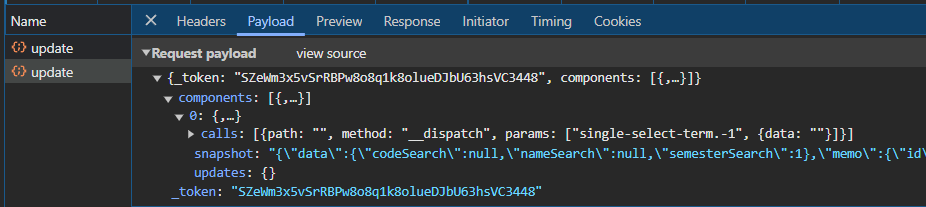
\includegraphics[width=15cm]{../pictures/screenshots/livewire_update.png}
	\caption{Livewire komponens frissítése: interakció esetén egy ilyen kérés kerül létrehozásra, ahol a \emph{snapshot} tartalmazza a komponens állapotát, amit újra ki kell értékelni.}
	\label{livewireUpdate}
\end{figure}

\subsection{Komponensek és data binding}

Ahogy ez fentebb említettem, a csomag használatához komponenseket kell létrehozni, melyek egy PHP osztályból, és az ahhoz tartozó nézetből állnak. Az osztályban létrehozott mezőkhöz és függvényekhez hozzá tudunk férni a nézetünkben, és akár hozzá is tudjuk ezeket az értékeket kötni egyes beviteli mezőkhöz a \emph{wire:model} segítségével. A függvények meghívásait pedig gombnyomásokhoz, vagy űrlapok elküldéséhez is köthetjük a \emph{wire:click} és \emph{wire:submit} használatával. Így amikor a felhasználó begépel valamit egy mezőbe, és/vagy megnyom egy gombot, a mögöttes PHP osztály állapota frissül, ez kerül elküldésre \aref{livewireUpdate}. kódrészletben látható módon, amit kiértékel a szerver, és visszaküldi. Ezek a komponensek egyébként Blade fájlok egyben, így \aref{bladeSection}. fejezetben írt direktívák továbbra is használhatók. Amennyiben azt szeretnénk, hogy minden  gombnyomásra frissüljön az oldal-- ez akkor hasznos például, ha az űrlap kitöltése során egyből szeretnénk frissíteni az oldalt esetleges hibaüzenetekkel --, akkor ezt is megtehetjük, ha a direktívát kiegészítjük a \emph{live} kulcsszóval.

\lstinputlisting[caption={A komponens osztályának egy mezője és egy bemeneti mező összekapcsolása, ami a harmadik sorban található.}, label=binding, style=php]{../codes/binding.blade.php}

A programomban főként ilyen Livewire komponenseket használtam . Ez alól egyedül a bejelentkezés és a regisztráció képez kivételt, mivel azokhoz \aref{fortifyAuth}. fejezetben írt csomagot használtam, és ott sima Blade fájlokkal kellett dolgozni.

\subsection{Livewire és SPA}

A fentebb említettek alapján sikerült kialakítani dinamikusan frissülő nézeteket, viszont egy probléma továbbra is fent állt: az oldalak közötti navigáció esetén továbbra is az egész oldal újra töltődött. Ennek megoldására találták ki a Livewire \emph{Navigate}\cite{navigate} funkcióját. Használata egyszerű: a navigálásra szánt gombokra, hivatkozásokra a \emph{wire:navigate} direktívát kell alkalmazni. Ezután amikor rákattint a felhasználó, az oldal teljes újratöltése helyett a háttérben kéri le a weboldalt a szervertől, majd a kapott adatok alapján módosítja a dokumentum struktúráját a Livewire.

Ezáltal egy SPA típusú oldal hozható létre, melynek jelentése: Single Page Application, avagy Egy oldalból álló alkalmazás. Ahogy a neve is sugallja, ezek olyan alkalmazások, amik egy oldalt töltenek be teljesen, a későbbiek során ennek az oldalnak a felépítését módosítják háttérben történő kérésekkel, mint ami \aref{livewireUpdate}. ábrán is látható.\cite{spa}

\subsection{Események}
\label{livewireevents}
A csomag lehetőséget ad események küldésére és fogadására is. Ezt én elsősorban kettő funkció megoldására használtam fel. Az egyik a legördülő kiválasztó mezők esetén volt. Ezek a mezők külön komponensek, így amikor annak az értéke frissül, akkor egy eseményt hozok létre, amit fogad az a komponens, amibe a mező be van ágyazva, ezáltal módosítva az értéket. A másik ilyen a felugró ablakok bezárása: ha valamilyen modell létrehozására szolgáló felugró ablakot nyit meg a felhasználó, majd a mezők megfelelő kitöltése után a mentésre kattint a felhasználó, akkor -- amennyiben nem lép közbe validációs probléma -- a mentést megvalósító függvény egy eseményt küld, hogy záródjon be az ablak.

Ilyen eseményeket a komponensben belül a \emph{dispatch()} függvény segítségével küldhetünk, ahol adni kell egy nevet az eseménynek, illetve igény szerint egyéb adatokat, amiket szeretnék mellékelni az eseményhez.

Az eseményeket fogadni többféleképpen tudjuk. Például a legördülő mezők esetén közvetlen a komponens osztályában fogadtam az eseményt. Ehhez egy függvényt kellett írni, aminél az \emph{\#On} attribútumot kellett alkalmazni. Amennyiben egyéb adatok is várunk az eseménynél, akkor azt a függvény paraméterein keresztül tudjuk megkapni. Ezt felhasználva, amikor változott a legördülő mező értéke, akkor egy eseményben kiküldtem a szülő komponensnek az új értéket, azt ő fogadta, és eltárolta azt.

Eseményt nem csak a PHP kódban, hanem a nézetekben, JavaScript-ben belül is tudunk fogadni. Ez a felugró ablakok bezárásánál volt előnyös, hiszen a nézetből férek hozzá az egyes HTML elemekhez az oldalon. Ilyenkor a JavaScript kódunkban a \emph{Livewire.on} függvényt kell használni, megadni az esemény nevét, illetve hogy mi történjen az esemény bekövetkezésekor, tehát jelen példában záródjon be az ablak.

\lstinputlisting[caption={Események küldése és fogadása.}, label=events, style=php]{../codes/events.php}

\subsection{WireToast: Livewire alapú értesítések}

Az utolsó Livewire-el kapcsolat téma, amit szeretnék megemlíteni, az az oldalon megjelenő értesítések egyes interakciók után, mint például létrehozás. Ehhez a \emph{Tall toasts}\cite{talltoasts} nevű csomagot használtam. Ez a Livewire-rel együtt működő csomag, így csak ilyen komponenseken belül lehet használni. Működéséhez a komponensek használnia kell a \emph{WireToasts} nevezetű trait-et, majd pedig a \emph{toast()} függvény meghívásával hozható létre ilyen értesítés. Ezután a típusát kell megadni (információ, siker, esetleg hiba), illetve a megjelenítendő szöveget és címet. Majd a \emph{push()} függvénnyel tudjuk kiküldeni az értesítést.

\lstinputlisting[caption={Oldalon megjelenő sikeres értesítés küldése.}, label=wiretoast, style=php]{../codes/toast.php}

Az értesítések kinézete természetesen személyre szabható, én például a DaisyUi által szolgáltatott értesítés komponensre írtam át az eredeti nézeteket.

\begin{figure}[ht!]
	\centering
	
\includegraphics[width=10cm]{../pictures/screenshots/notif.png}
	\caption{A létrejövő értesítés kinézete.}
	\label{toastUI}
\end{figure}

\section{Websocket és Pusher}

Amikor \aref{class}. képen látható oldalt készítettem, akkor mindenképpen szerettem volna megoldani, hogy amikor a tanuló a Qr kód segítségével bejelentkezik az órára, a státusza automatikusan frissüljön a tanár által látott oldalon is. Első gondolatom az volt, hogy periodikusan, pár másodpercenként frissítem az oldalt, viszont ezt az ötletet hamar elvetettem, mivel ez rengeteg fölösleges kéréssel járna, ami sok töltést jelentene a felhasználóknak, illetve terhet a szervernek. Így másik megoldás után néztem, ekkor találtam rá a Websocket-ekre és a Pusher szolgáltatásra.

\subsection{Websocket}

A Websocket technológia kétirányú kommunikációt tesz lehető a szerver és a kliensek között. Ezáltal a folytonos frissítést, amit először terveztem, eseményekkel lehet kiváltani.\cite{websocket}Amikor valaki bejelentkezik az órára, akkor egy esemény jön létre, ezt a tanári oldal fogadja, és innen tudja, hogy frissíteni kell az adott tanulóhoz tartozó sort. Ezek nem azok az események, amiket \aref{livewireevents}. fejezetben taglaltam. Azok az események az adott felhasználói munkamenetre korlátozódnak, míg ezek az események küldése, fogadása eszközök, felhasználók között történnek.

\subsection{Pusher channels}

A Pusher Channels\cite{pusher} tulajdonképpen egy megvalósítása a Websocketeknek, amit kifejezetten webalkalmazásokhoz terveztek. Ingyenes fiókot lehet hozzá létrehozni, ami bár korlátolt, a szakdolgozat készítéséhez és kipróbálásához bőven elegendő. A Laravel keretrendszer is támogatja a Pusher technológiát, így könnyen integrálható volt a programba. Mondhatni a Pusher a szerver és a kliensek között áll: ide érkeznek be az események, és innen kerülnek kiküldésre.

Természetesen más, akár nyílt forrású megoldások is elérhetők, illetve a dolgozat készítésekor is fejlesztés alatt volt egy kifejezetten a Laravel-hez készülő változat, viszont a fejlesztők későn lettek készek vele ahhoz, hogy fel tudjam használni szakdolgozatomban, így a Pusher lecserélése erre a megoldásra egy jövőbeli feladat lesz.

\subsection{Csatornák, események létrehozása}

A Websocketek konfigurálása és használata két részre tehető: a szerver és a kliens beállítására és az ezekhez szükséges csomagok telepítésére.

Pusher használata esetén regisztrálnunk kell magunkat, majd a kapott hozzáférési kulcsokat és adatokat megadni a környezeti fájlban, illetve engedélyezni kell az események közvetítését a konfigurációs fájlokban. Végezetül a Pusher-hez szükséges csomag telepítését kell elvégezni, illetve beállítani -- szintén a környezeti fájlban --, hogy a közvetítésre a Pusher-t használjon a keretrendszer. Szükséges még egy sor(Queue) beállítása is, mivel innen kerülnek az események kiküldésre, de mivel az emailek esetén is szükség volt erre, így ezzel a lépéssel már készen voltam.\cite{broadcasting}

Ezután készen állunk az események létrehozására. A jelenlét megváltozására létrehoztam a \emph{ClassPresenceChanged} eseményt. Ez az esemény kerül kiküldésre ha a hallgató bejelentkezik az órára a QR kódon keresztül. Az osztálynak implementálnia kell a \emph{ShouldBroadcast} interfészt, ami egy függvényt tartalmaz, a \emph{broadcastOn} függvényt. Itt kell definiálunk azon csatorná(ka)t, ahol szeretnék az eseményt hirdetni. Lehetőség van privát csatornák létrehozására is, de nekem elegendő volt a publikus csatorna is ebben az esetben. Az eseményeket a \emph{updatePresence} csatornánkon hirdetem, amihez hozzáfűzöm a jelenlétet leíró entitás azonosítóját, ez látható \aref{broadcastOn}. részletben. Hogy ezt megtehessem, az esemény osztályának konstruktorában bekérem a jelenlét entitást. Így minden tanuló minden órájához külön csatorna tartozik azért, hogy az óránál egyszerre csak egy sor frissüljön, ne az összes mindig.
\pagebreak

\lstinputlisting[caption={Csatorna definiálása az esemény osztályában.}, label=broadcastOn, style=php]{../codes/event.php}

Az események létrehozása után az osztálynevük, majd a \emph{dispatch} függvényhasználatával, illetve az esetleges konstruktor értékek megadásával küldhetjük el az eseményt.

\lstinputlisting[caption={Esemény elküldése.}, label=sendEvent, style=php]{../codes/sendEvent.php}

\subsection{Események fogadása JavaScript, LiveWire esetén}

Természetesen ezeket az eseményeket fogadni is kell. Ehhez nyújt megoldást a Laravel Echo\cite{broadcasting}. Itt is szükséges maga az Echo és a Pusher-hez tartozó csomagok telepítése. Ezek után egy Echo példányt kell létrehoznunk a JavaScript kódunkban. Ez a példány kapja meg a csatornákhoz való csatlakozás adatait, és ez fogja fogadni az eseményeket. A keretrendszer alapból tartalmaz egy ilyen példányt, amit csak ki kell vennünk a  kommentekből. Az autentikációs adatokat a környezeti fájlból kiolvassa, így ez használatra kész.

Az Echo példány létrehozása után JavaScript kódból tudunk az eseményekre figyelni, viszont én nem ezt az utat választottam. Helyette Livewire komponensből figyeltem az eseményeket. Ehhez továbbra is szükség van a Laravel Echo csomagra az események fogadásához, viszont azt, hogy mi történik, és hogy milyen csatornákat, eseményeket figyelek, azt már a PHP osztályon belül tudom megadni, hasonlóan \aref{livewireevents}. alfejezetben írt módon.

Továbbra is az \emph{\#On[]} attribútumot kell alkalmazni, viszont az esemény leírásában az \emph{echo} előtagot, a csatorna nevét, majd az esemény nevét kell leírni.\cite{livewireEcho}. Az esemény nevénél szükség lehet az egész névteret megadni, ahol az esemény osztálya található.

\lstinputlisting[caption={Esemény fogadása Livewire komponensből. A \emph{pivot.id} helyére az osztály \emph{pivot} mezőjének \emph{id} értéke kerül behelyettesítésre. Esemény érkezésekor frissítem az adatokat, és egy másik eseménnyel a diagrammot.}, label=getEvent, style=php]{../codes/receiveEvent.php}

\section{Progressive Web Apps}

Az alkalmazás elkezdése előtt azért döntöttem a weboldal mellett, mivel ez a legkönnyebb módon elérhető alkalmazás, hiszen telepíteni se kell. Ugyan akkor a fejlesztés során elgondolkoztam, hogy jó lenne, ha akár telepíteni is tudnák a felhasználók az alkalmazást, hogy gyorsabban hozzáférjenek. Ezért is lett belőle PWA alkalmazás.

A PWA, avagy a Progressive Web Apps olyan webalkalmazások, melyek webes technológiákkal készültek, webböngészőkben futnak, de képesek platform specifikus alkalmazásként is viselkedni, beépülni a rendszerbe.\cite{PWA} Ez a gyakorlatban azt jelenti, hogy az alkalmazás külön ablakban nyílik meg, nem a böngészőben, a telepített alkalmazások között megjelenik, illetve az is előfordulhat, hogy egyes részei internetkapcsolat nélkül is működnek.

Ennek megvalósításához a Laravel PWA\cite{laravelpwa} csomagot használtam. Ez a könyvtár segítség nyújt a \emph{manifest} fájl és a \emph{service worker} létrehozásában, melyek szükségesek a PWA működéséhez. A csomag létrehozza ezeket, illetve létrehoz egy oldalt is, ami akkor jelenik meg, ha nincs internetkapcsolat. Ezeket szabtam személyre.

Fontos megjegyezni, hogy a PWA alkalmazások csak HTTPS kapcsolat alatt működnek, ez alól kivételt a fejlesztői környezetben futó alkalmazások jelentenek csak. Sajnos egyedüli hátránya, hogy nem minden böngésző támogatja a PWA alkalmazások telepítését, de attól maga az oldal továbbra is működik.

\subsection{A manifest fájl}

A \emph{manifest} fájl tartalmazza az alkalmazás adatait, mint például a nevét is. Ezt a fájlt szükséges behivatkozni a főoldalon. A böngésző érzékeli ezt a fájlt, és innen tudja, hogy a weboldal telepíthető PWA alkalmazásként, illetve a telepített alkalmazás nevét, ikonját is innen szerzi be. \Aref{manytomany}. kódrészleten láthatjuk ezt a fájlt. Itt több beállítást meg lehet adni: az alkalmazás nevét, kezdő címét, háttér színét és az ikonjait, csak hogy párat kiemeljek. Vannak más lehetőségek is, amiket itt nem használtam, például más méretű ikonokat, vagy gyors parancsokat is fel lehet venni.

\lstinputlisting[caption={Az oldal által használt manifest fájl.}, label=manifest, style=jsonstyle]{../codes/manifest.json}

\subsection{Service Worker}

A másik fontos összetevő a a Service worker. Ennek az egyik fő feladata, hogy gyorsító tárazza az oldal egyes elemeit. Az oldal betöltésekor regisztrálja magát, és elmenti a gyorsítótárba a fájlokat. Ezáltal akkor is működni tud, ha nincs kapcsolat a szerverrel. Ezt a szolgáltatását arra használtam ki, hogy egy személyre szabott oldalt jelenítsek meg kapcsolat hiányának esetén. Ez úgy történik, hogy minden kérést és választ megvizsgál a service worker. Amennyiben úgy látja, hogy a szerver nem elérhető, akkor a gyorsítótárból tölti be a hibát jelző oldalt, ellenkező esetben pedig tovább engedi a kérést. 

Sajnos az oldal többi részén használt Tailwind-et itt nem tudtam alkalmazni, mivel a stílusokat tartalmazó fájlok minden újraépítés során kapnak egy egyedi azonosító részt, így nem tudtam őket felvenni a gyorsítótárazandó fájlok közé. Ezért ezen az ,,offline'' oldalon a BootStrap-et\cite{bootstrap} alkalmaztam, amely egy másik komponens keretrendszer, mivel az ehhez szükséges fájlt csak be raktam a publikusan elérhető fájlok közé, és ezt már sikerült gyorsítótárazni.

\lstinputlisting[caption={Részlet a Laravel PWA csomagból származó service worker fájlból.\cite{laravelpwa}}, label=service, style=js]{../codes/service_worker.js}

\section{Egyéb csomagok}

\subsection{Qr kód generálás}

A Qr kódok olyan kétdimenziós, négyzetes képek, amiket azok gyors, kamerával való beolvasására fejlesztettek ki.\cite{qrCodeWhatIsIt} Amikor egy gyorsabb módszeren gondolkoztam, amivel bejelentkezhetnek a diákok az órákra, és nem szükséges hozzá különösebb eszköz, akkor végül ezen kódok használata mellett döntöttem, hiszen a tanárnak csak ki kell ezt vetíteni, a hallgatók pedig telefonjukkal be tudják azt szkennelni.

A QR kódok generálására a \emph{Simple QrCode}\cite{qrCode} nevű csomagot használom. Telepítés után a Blade fájlban közvetlen létre tudjuk hozni a kódot, ahol a méretét, és a kódolandó szöveget kell megadni.

\lstinputlisting[caption={Qr kód generálása 250-es mérettel, ami a bejelentkező linket tartalmazza, ezt a komponens egyik mezőjéből kértem le.}, label=qr, style=php]{../codes/qr.blade.php}

\subsection{Naptár - FullCalendar.js}

Az órarend megjelenítésére használtam a FullCalendar.js\cite{fullcalendar} nevezetű csomagot. Ez egy nagyon személyre szabható csomag, a színek, méretek, felépítések is testre szabhatók. Beállítható a nyelv, a megjelenő napok száma és az események kinézete is többek között.

Mivel ez egy JavaScript alapú csomag, így az órarend létrehozása is azzal történt, ennek kódja a Blade komponens-be van beágyazva. Ez viszont egy problémát hozott magával: az órarendben megjelenő eseményeket a PHP kód szolgáltatja, így a kettőt össze kellett valamilyen módon kötni. Szerencsére sikerült megoldást találnom. A Livewire lehetővé teszi, hogy a PHP komponensben található függvényeket meghívjuk JavaScript kódunkban, és azoknak visszatérési értékét feldolgozzuk. a FullCalender csomag pedig lehetőséget nyújt arra, hogy amennyiben a naptár megjelenítésre kerül, vagy másik időtartományra vált a felhasználó, akkor egy JavaScript függvény fusson le, ami elvégzi a kiválasztott időtartamban található események lekérdezését. Bár ezt elsődlegesen API végpontok meghívására tervezték, jól működik Livewire esetén is. Ilyenkor meghívásra kerül a PHP függvény, ami megkapja a kiválasztott időtartamot, lekérdezi az adatbázisból a felhasználó óráit, ezeket egy asszociatív tömbbe gyűjti, majd vissza adja ezt. Az így kapott adatot a FullCalendar csomag fel tudja használni és megjeleníteni az órákat. Itt volt lehetőség megadni azt is, hogy milyen színe legyen az eseménynek, így azt is könnyű volt megoldani, hogy attól függően, hogy milyen a státusza a hallgatónak az órán, változik a színe.

Ez a megoldás még egy pozitívumot vont magával, amibe először nem is gondoltam bele, csak utólag. Amikor új eseményekre van szüksége a naptárnak, akkor ezek lekérésekor megadja azt is, hogy mely napok láthatóak jelenleg az oldalon, amit tovább lehet küldeni a PHP függvénynek paraméterként. Így nem kell az órarend megnyitásakor a felhasználó összes óráját lekérdezni, elég csak egy részét, ami nagy teljesítménybeli ugrást jelenthet, ha már több félév adata is benne van az adatbázisban.

\lstinputlisting[caption={Események lekérdezése. A második sorban látható a \emph{getEvents} nevű PHP függvény meghívása.}, label=eventGet, style=js]{../codes/calendarEvent.js}

\subsection{Diagramok - Chart.js}

A főoldalon és az óráknál megjelenő diagramokat a Chart.js\cite{chartjs} nevezet könyvtárral készítettem el, ami szintén a nagy személyre szabhatóság  miatt tetszett meg. Sok különböző típusú diagramot támogat, de nekem leginkább a kördiagramok létrehozására használtam fel. A fent említett probléma itt is megjelent, mely szerint a PHP szolgáltatja az adatokat, viszont itt egyszerűbb volt a megoldás, tekintettel arra, hogy csak pár számot kell a diagramnak megkapnia, nem egész eseményeket. Blade direktívák segítségével beleírtam a komponens nézetbe -- ami tartalmazza a diagram létrehozására szolgáló JavaScript kódot is --, hogy milyen értékeket kell megjeleníteni a kördiagramnak. Illetve ugyan itt figyelek egy \emph{updateChart} eseményre, ami megkapja friss adatokat, és átírja  a diagram-on az értékeket, így a frissítés is meg van oldva.

\lstinputlisting[caption={Részlet egy kördiagram létrehozásából.}, label=chart, style=js]{../codes/chart.js}

\chapter{Az alkalmazás tesztelése}
\label{testing}
\section{Manuális tesztelés}
\section{Automatizált tesztelés}
\section{Terheléses tesztelés}
\section{Laravel Pint és Github actions}

\chapter{Alkalmazás telepítése}
\label{setup}
Az alkalmazás a szakdolgozat védés, illetve a záróvizsga időszak alatt elérhető a \url{https://szakdolgozat.ddns.net} címen, ahol ki lehet próbálni az alkalmazást. Pár alapértelmezett felhasználó elérhető:
\begin{itemize}
	\item Szuper adminisztrátor:
	\begin{itemize}
		\item Felhasználónév: \emph{SADMIN}
		\item Jelszó: \emph{superadmin}
	\end{itemize}
	\item Adminisztrátor:
	\begin{itemize}
		\item Felhasználónév: \emph{ADMIN0}
		\item Jelszó: \emph{admin}
	\end{itemize}
	\item Tanár:
	\begin{itemize}
		\item Felhasználónév: \emph{TEACHE}
		\item Jelszó: \emph{teacher}
	\end{itemize}
	\item Hallgató:
	\begin{itemize}
		\item Felhasználónév: \emph{STUDEN}
		\item Jelszó: \emph{student}
	\end{itemize}
\end{itemize}
\section{Laravel Forge}
\section{Kézi telepítés lépései}
\begin{enumerate}
	\item Töltsük le az alkalmazás fájljait.
	\item A futtatáshoz szükségünk van egy adatbázis szerverre. Javasolt MySQL vagy PostgreSQL használata. Ezeknek a telepítéséről az adott adatbázisszerver weboldalán lehet tájékozódni.
	\item Telepítsük a PHP-t számítógépünkre, legalább a 8.1-es verziót, melyet a Laravel keretrendszer 10-es verziója követel meg. Alternatívaként telepíthetjük a XAMPP nevezetű programot is, mely feltelepít egy adatbázis és PHP disztribúciót is.
	\item Konfiguráljuk az adatbázist: hozzunk létre egy felhasználót és egy sémát, amihez hozz fog tudni férni az oldalunk.
	\item Az alábbi php kiegészítő csomagok engedélyezése szükséges: Ctype, cURL, DOM, Fileinfo, Filter, Hash, Mbstring, OpenSSL, PCRE, PDO, Session, Tokenizer, XML.
	\item Telepítsük a Composer nevű PHP csomagkezelő rendszert.
	\item Telepítsük a Node.js nevű JavaScript futtatókörnyezetet.
	\item A sikeres telepítések után navigáljunk el a \emph{thesisproject} nevű mappába a letöltött fájlok között. Ez tartalmazza a program fájljait, a továbbiakban itt dolgozunk, itt adunk ki parancsokat.
	\item Készítsünk egy másolatot a \emph{.env.example} nevű fájlról és nevezzük azt át \emph{.env} névre. Nyissuk meg, és töltsük ki az alábbi adatokat:
	\begin{itemize}
		\item APP\_URL: amennyiben nem helyi környezetben, kipróbálásra telepítjük, akkor itt adjuk meg az alkalmazás elérési útját.
		\item DB prefixummal kezdődő értékek: itt állítsuk be az adatbázis kapcsolat adatait.
		\item BROADCAST\_DRIVER: értékét állítsuk át \emph{pusher}-re.
		\item QUEUE\_CONNECTION: értékét állítsuk át \emph{database}-re, amennyiben az adatbázist szeretnék használni a sor-hoz.
		\item MAIL prefixummal kezdődő értékek: itt állíthatjuk be a levelezéshez használt hozzáférési értékeket. Ezekről az email szolgáltatótól kaphatunk információt.
		\item PUSHER prefixummal kezdődő értékek: itt a Pusher hozzáférési adatok beállítása szükséges. Ezekhez fiókot kell regisztrálnunk, miután elérhetővé válnak a szükséges értékek. 
	\end{itemize}
	A többi értéket az alkalmazáson belül tudjuk módosítani.

	\item Ezek után a csomagok telepítése szükséges. Adjuk ki a terminálban a \textbf{composer install -\/-optimize-autoloader -\/-no-dev} parancsot.
	\item Majd pedig a \textbf{npm ci} és az \textbf{npm run build} parancsokat.
	\item Ezek után az alábbi parancsok kiadása szükséges:
	\begin{itemize}
		\item \textbf{php artisan key:generate}: alkalmazás kulcs generálása.
		\item \textbf{php artisan migrate -\/-seed}: adatbázis felépítése.
		\item \textbf{php artisan route:cache}: útvonalak gyorsítótárazása.
		\item \textbf{php artisan config:cache}: konfiguráció gyorsítótárazása.
		\item \textbf{php artisan storage:link}: a képek tárolására használt könyvtár elérhetővé tétele.
		\item A keretrendszerben jártas olvasó észreveheti, hogy kihagytam a nézetek gyorsítótárazására szolgáló parancsot. A Livewire általam használt verziójában van egy olyan probléma, miszerint gyorsítótárazás esetén az egyes elemek nem működnek megfelelően. Ennek kiküszöbölésére döntöttem úgy, hogy a nézeteket nem gyorsítótárazom.
	\end{itemize}
	\item A fejlesztői szerver elindítható a \textbf{php artisan serve} paranccsal. Ugyan csak szükséges a sor elindítása is egy másik terminál ablakban: \textbf{php artisan queue:work}.
	\item Az alkalmazást megnyithatjuk a böngészőben, az alapértelmezett \textbf{SADMIN/superadmin} kombinációval tudunk belépni.
\end{enumerate}

\chapter*{Összegzés}
\addcontentsline{toc}{chapter}{Összegzés}

\begin{thebibliography}{19}
\addcontentsline{toc}{chapter}{\bibname}

\bibitem{Neptun}
\textsc{SDA Informatika Zrt:} \emph{Neptun alkalmazás leírása}
\\
\url{https://sdainformatika.hu/termekek}, Megtekintés dátuma: 2024.03.21.

\bibitem{ICS}
\textsc{FileInfo.com}: \emph{ICS fájl leírása.}
\\
\url{https://fileinfo.com/extension/ics}, Megtekintés dátuma: 2024.03.21.

\bibitem{PWA}
\textsc{MDN web docs}: \emph{Progressive web apps}
\\
\url{https://developer.mozilla.org/en-US/docs/Web/Progressive_web_apps}, Megtekintés dátuma: 2024.03.21.

\bibitem{QR}
\textsc{Kaspersky}: \emph{QR Code Security: What are QR codes and are they safe to use?}
\\
\url{https://www.kaspersky.com/resource-center/definitions/what-is-a-qr-code-how-to-scan}, Megtekintés dátuma: 2024.03.21.

\bibitem{meetlaravel}
\textsc{Laravel}: \emph{Meet Laravel}
\\
\url{https://laravel.com/docs/11.x#meet-laravel}, Megtekintés dátuma: 2024.03.24.

\bibitem{livewire}
\textsc{Livewire}: \emph{Főoldal}
\\
\url{https://livewire.laravel.com/}, Megtekintés dátuma: 2024.03.24.

\bibitem{routing}
\textsc{Livewire}: \emph{Routing}
\\
\url{https://laravel.com/docs/10.x/routing}, Megtekintés dátuma: 2024.03.24.

\bibitem{middleware}
\textsc{Livewire}: \emph{Middlewares}
\\
\url{https://laravel.com/docs/10.x/middleware}, Megtekintés dátuma: 2024.03.24.

\bibitem{mvc}
\textsc{MDN web docs}: \emph{MVC}
\\
\url{https://developer.mozilla.org/en-US/docs/Glossary/MVC}, Megtekintés dátuma: 2024.03.24.

\bibitem{blade}
\textsc{Laravel}: \emph{Blade templates}
\\
\url{https://laravel.com/docs/10.x/blade}, Megtekintés dátuma: 2024.03.24.

\bibitem{migrations}
\textsc{Laravel}: \emph{Database: Migrations}
\\
\url{https://laravel.com/docs/10.x/migrations}, Megtekintés dátuma: 2024.03.24.

\bibitem{tableNames}
\textsc{Laravel}: \emph{Eloquent: Table Names}
\\
\url{https://laravel.com/docs/10.x/eloquent#table-names}, Megtekintés dátuma: 2024.03.24.

\bibitem{magicMethod}
\textsc{PHP}: \emph{Magic Methods}
\\
\url{https://www.php.net/manual/en/language.oop5.magic.php}, Megtekintés dátuma: 2024.03.24.

\bibitem{orm}
\textsc{FreeCodeCamp}: \emph{What is an ORM – The Meaning of Object Relational Mapping Database Tools}
\\
\url{https://www.freecodecamp.org/news/what-is-an-orm-the-meaning-of-object-relational-mapping-database-tools/}, Megtekintés dátuma: 2024.03.25.

\bibitem{eloquentORM}
\textsc{Laravel}: \emph{Eloquent}
\\
\url{https://laravel.com/docs/10.x/eloquent}, Megtekintés dátuma: 2024.03.25.

\bibitem{blade}
\textsc{Laravel}: \emph{Blade Templates}
\\
\url{https://laravel.com/docs/10.x/blade}, Megtekintés dátuma: 2024.03.25.

\bibitem{fortify}
\textsc{Laravel}: \emph{Laravel Fortify}
\\
\url{https://laravel.com/docs/10.x/fortify}, Megtekintés dátuma: 2024.03.25.

\bibitem{ladder}
\textsc{Github}: \emph{Ladder}
\\
\url{https://github.com/eneadm/ladder}, Megtekintés dátuma: 2024.03.25.

\bibitem{policies}
\textsc{Laravel}: \emph{Creating Policies}
\\
\url{https://laravel.com/docs/10.x/authorization#creating-policies}, Megtekintés dátuma: 2024.03.25.

\bibitem{mail}
\textsc{Laravel}: \emph{Mail Notifications}
\\
\url{https://laravel.com/docs/10.x/notifications#mail-notifications}, Megtekintés dátuma: 2024.03.25.

\bibitem{icsFormat}
\textsc{WebDavSystem}: \emph{Calendar (.ics) File Structure}
\\
\url{https://www.webdavsystem.com/server/creating_caldav_carddav/calendar_ics_file_structure/}, Megtekintés dátuma: 2024.03.25.

\bibitem{tailwind}
\textsc{Tailwind}: \emph{Főoldal}
\\
\url{https://tailwindcss.com/}, Megtekintés dátuma: 2024.03.25.

\bibitem{daisyui}
\textsc{DaisyUI}: \emph{Főoldal}
\\
\url{https://daisyui.com/}, Megtekintés dátuma: 2024.03.25.

\bibitem{heroicons}
\textsc{Heroicons}: \emph{Főoldal}
\\
\url{https://heroicons.com/}, Megtekintés dátuma: 2024.03.25.

\bibitem{dom}
\textsc{MDN web docs}: \emph{Introduction to the DOM}
\\
\url{https://developer.mozilla.org/en-US/docs/Web/API/Document_Object_Model/Introduction}, Megtekintés dátuma: 2024.03.26.

\bibitem{navigate}
\textsc{Livewire}: \emph{Navigate}
\\
\url{https://livewire.laravel.com/docs/navigate}, Megtekintés dátuma: 2024.03.26.

\bibitem{spa}
\textsc{MDN web docs}: \emph{SPA (Single-page application)}
\\
\url{https://developer.mozilla.org/en-US/docs/Glossary/SPA}, Megtekintés dátuma: 2024.03.26.

\bibitem{spa}
\textsc{Livewire}: \emph{Events}
\\
\url{https://livewire.laravel.com/docs/events}, Megtekintés dátuma: 2024.03.26.

\bibitem{talltoasts}
\textsc{Github: usernotnull}: \emph{Tall toasts}
\\
\url{https://github.com/usernotnull/tall-toasts}, Megtekintés dátuma: 2024.03.26.

\bibitem{websocket}
\textsc{MDN web docs}: \emph{The WebSocket API (WebSockets)}
\\
\url{https://developer.mozilla.org/en-US/docs/Web/API/WebSockets_API}, Megtekintés dátuma: 2024.03.26.

\bibitem{pusher}
\textsc{Pusher}: \emph{Pusher channels}
\\
\url{https://pusher.com/channels/}, Megtekintés dátuma: 2024.03.26.

\bibitem{broadcasting}
\textsc{Laravel}: \emph{Broadcasting}
\\
\url{https://laravel.com/docs/10.x/broadcasting}, Megtekintés dátuma: 2024.03.28.

\bibitem{livewireEcho}
\textsc{Livewire}: \emph{Real-time events using Laravel Echo}
\\
\url{https://livewire.laravel.com/docs/events#real-time-events-using-laravel-echo}, Megtekintés dátuma: 2024.03.28.

\bibitem{qrCodeWhatIsIt}
\textsc{keyence.eu}: \emph{Mit nevezünk QR-kódnak?}
\\
\url{https://www.keyence.eu/huhu/ss/products/auto_id/codereader/basic_2d/qr.jsp}, Megtekintés dátuma: 2024.03.28.

\bibitem{qrCode}
\textsc{Github}: \emph{SimpleSoftwareIO: Simple QrCode}
\\
\url{https://github.com/SimpleSoftwareIO/simple-qrcode}, Megtekintés dátuma: 2024.03.28.

\bibitem{fullcalendar}
\textsc{FullCalendar}: \emph{Főoldal}
\\
\url{https://fullcalendar.io/}, Megtekintés dátuma: 2024.03.28.

\bibitem{chartjs}
\textsc{Chart.js}: \emph{Főoldal}
\\
\url{https://www.chartjs.org/}, Megtekintés dátuma: 2024.03.28.

\bibitem{laravelpwa}
\textsc{Github}: \emph{silviolleite: laravel-pwa}
\\
\url{https://www.chartjs.org/}, Megtekintés dátuma: 2024.03.28.

\bibitem{bootstrap}
\textsc{Bootstrap}: \emph{Főoldal}
\\
\url{https://getbootstrap.com/}, Megtekintés dátuma: 2024.03.28.

\end{thebibliography}

%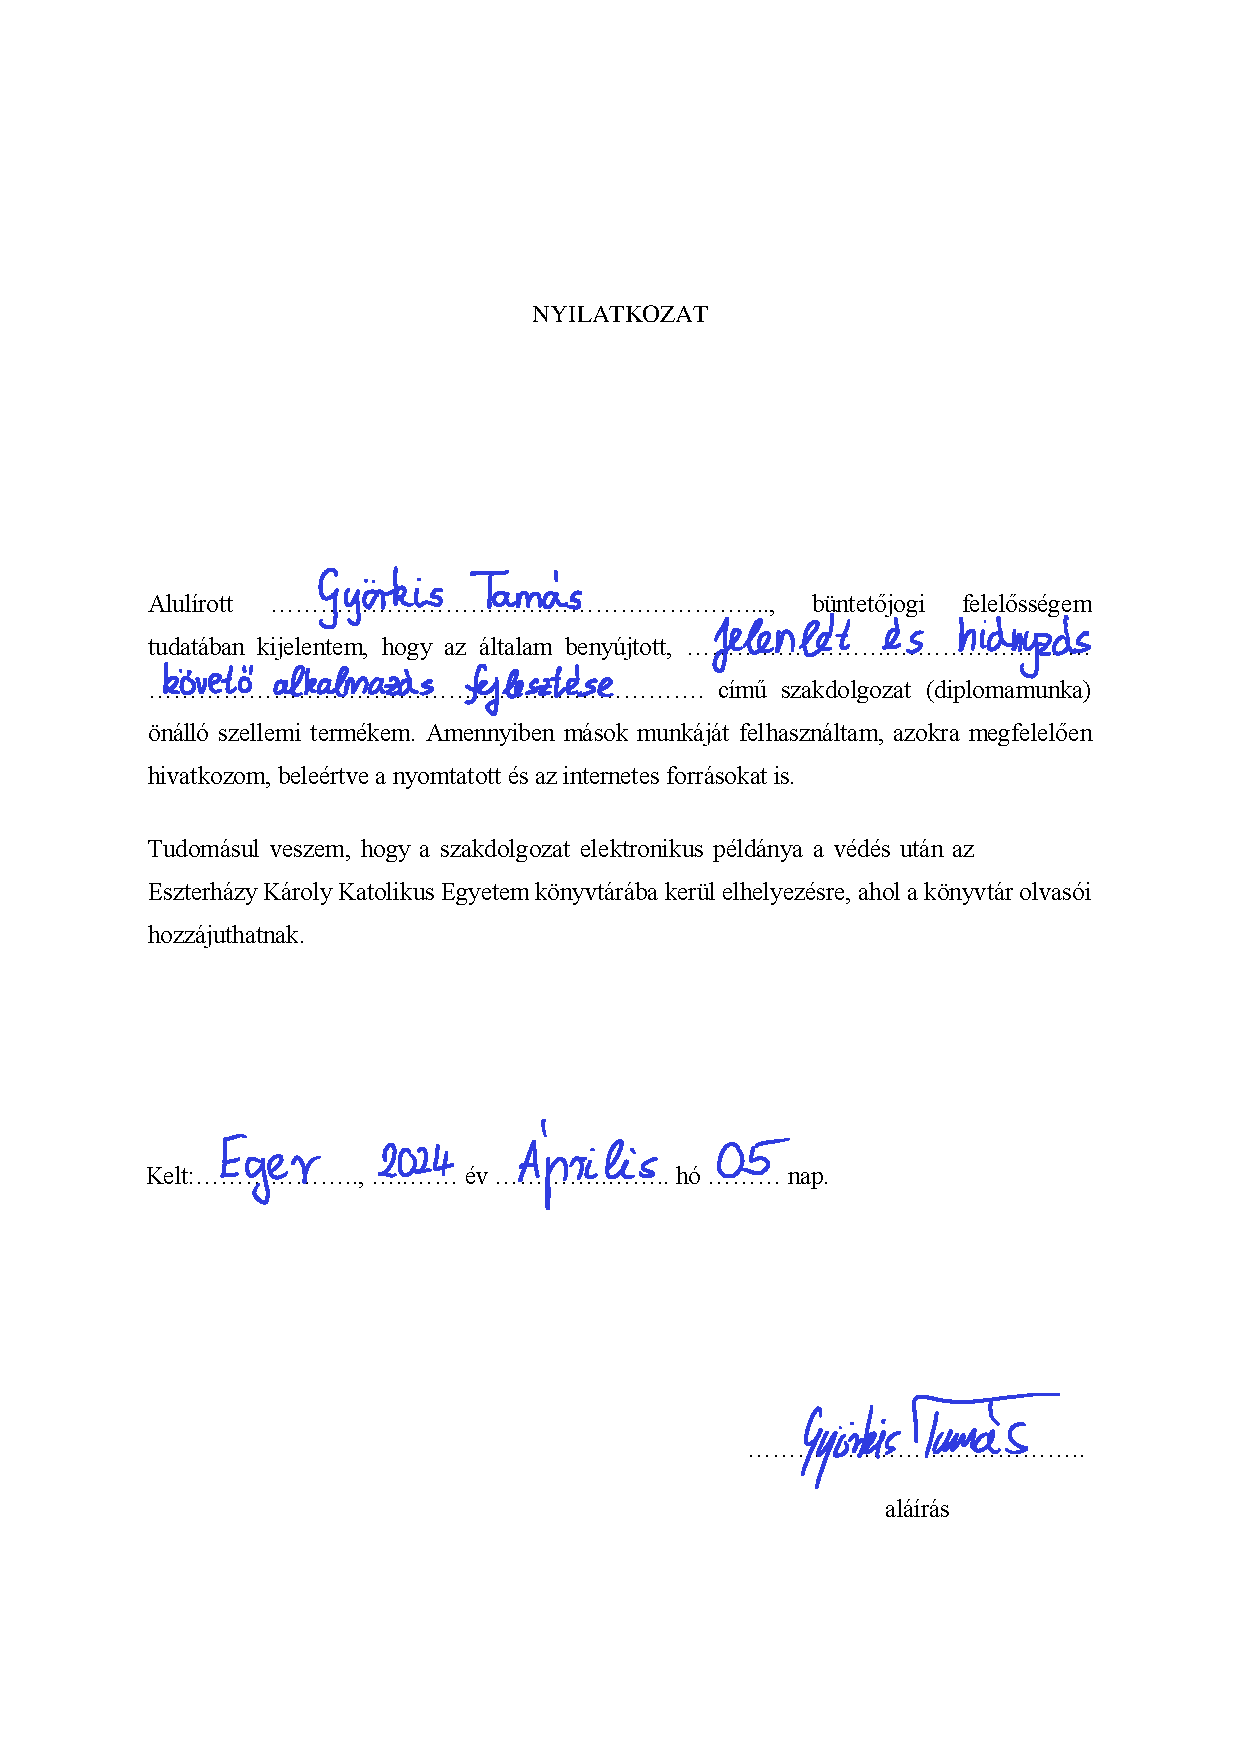
\includepdf{nyilatkozat.pdf}
\end{document}